\chapter {Network Architecture}

Since the task of image segmentation is a popular one, a number of architecture propositions have been made that aim to produce segmentations. Among them is the \textit{U-Net}, which is the basis of the network used in this thesis.  In the following sections, the principles behind so-called Convolutional Neural Networks, the differences between them and normal MLPs and the operations in such networks are detailed.


	\section{Convolutional Neural Networks}
\label{sec:CNN}
\textit{Convolutional Neural Networks} (CNNs) are a special subtype of ANNs/MLPs that was popularized by LeCun \cite{lecun98} and, more recently, the successes of Krizhevsky \cite{krizhevsky2012} in the domain of image classification, although CNNs have been applied to other problems such as sound analysis as well. The rationale for their creation was that using fully-connected networks like the ones presented in section \ref{subsec:mlp_backprop} relate all elements of an input vector to every other element, which is generally a good thing to do - however, it ignores the relationship between parts of the input that is given in some datasets and doesn't scale well for very large datasets because of the large number of weights needed. Especially in image data, pixels that are close to each other by some metric such as the Euclidean distance are much more likely to be related, while pixels that lie on the other side of the image hardly are relevant in the context of operations like pixel classification. Consequently, CNNs encode this spatial relationship by using convolution operations. Concretely, a convolution layer in a CNN typically consists of three sub-components:\\

\noindent First, the data is convoluted by applying one or multiple kernels (also called filter) to all input values and their local neighborhoods.\footnote{Although the convolution in section \ref{sec:canny} describes out-of-bounds handling, the architecture used in this thesis uses only the naturally valid part of the convolution, i.e. if a $3 \times 3 \times d$ filter is used, a 1-value border of the data is lost because the local neighborhood would be partly out of bounds for these border values.} Kernels typically have a size of $k \times k \times d$, where $k$ is the filter size and $d$ is the depth of the dataset, e.g. in an RGB image dataset, the depth is 3 because there are 3 color channels. The result of these convolutions are as many outputs, called \textit{feature maps}, as there are filters in the layer. When viewed as a graph, this means that the hidden neurons represent the results of each convolution step, while all hidden neurons of the same filter share the same weights.

Effectively, this means that the same kind of pattern is searched in the entire dataset, resulting in \textit{translation invariance}, i.e. it doesn't matter where the pattern is because it is still the same pattern at every position in the data.

Then, the feature maps are passed through an non-linear activation function $h(\cdot)$, just like in normal MLPs, to generate activation maps.

\noindent Finally, these activation maps are exposed to a pooling operation such as \textit{Maximum Pooling}. Maximum pooling is a downsampling method that reduces the complexity of the network by replacing groups of values that are apart by a certain stride in the activation map with the maximum value within that group, resulting in a condensed activation map, while performing this calculation for each depth slice of the data independently. Intuitively, some of the information about where a pattern was detected by a filter while creating the feature map is given up in order to make the network easier to train, although the relative positions between patterns are kept intact. \cite[pp. 330-345]{deeplearning_book}\\

\noindent The training of such a network then proceeds like in an MLP, only that the weights that the network has to learn by backpropating the loss through the network are the weights of fully-connected layer as well as the filter weights.\\

\noindent See figure \ref{fig:convnet} for an example of a simple CNN architecture.

\begin {figure}[!ht]
	\begin{center}
		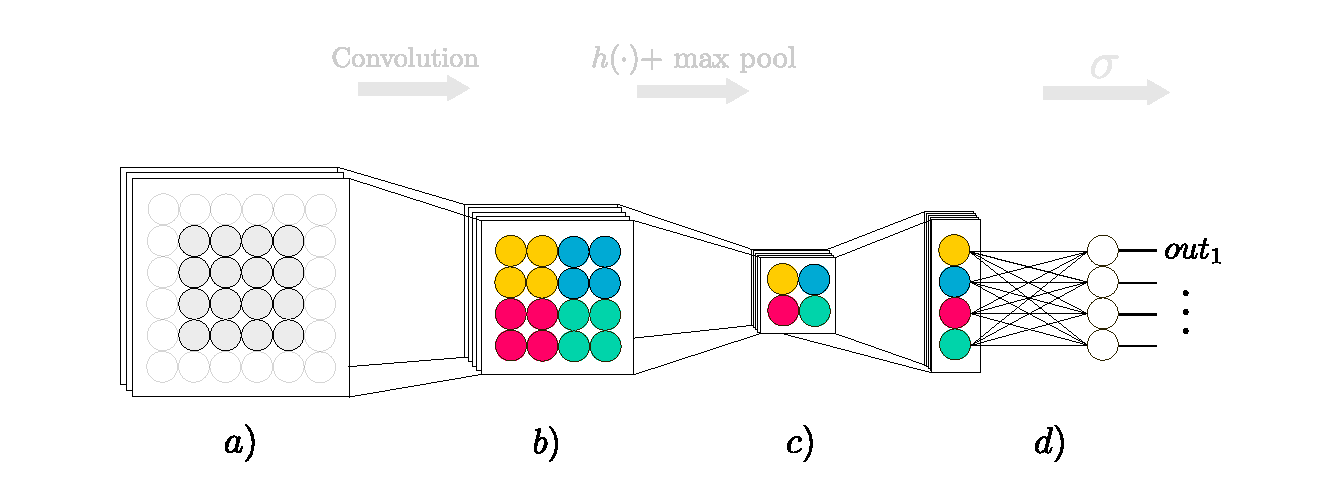
\includegraphics[scale=0.75]{img/fig_convnet}
	\end{center}
	\caption{A Convolutional Neural Network with multiple filters. For simplicity, most neuron connections aren't shown explicitly. \textbf{a):} Input layer. The input size is $6 \times 6 \times 3$, while the kernel size is $3 \times 3 \times 3$. Neurons with valid convolution neighborhoods shown in gray. \textbf{b):} Feature maps with size $4 \times 4 \times 3$ that are the result of applying convolution filters to the input, which are then passed into the activation function $h$ to create activation maps. \textbf{c):} Results of a Maximum Pooling operation with sizes $2 \times 2$ and stride $2$ applied to the activation maps. The colors indicate the downsampled position of the maximum activation in a pooling region. \textbf{d):} Fully-connected output layer that calculates the network outputs via applying the output function $\sigma$. The max-pooled values have been rearranged into a column for clarity, and connections are color-coded by the receiving neuron.}
	\label{fig:convnet}
\end {figure}


	\section {Activation Functions}
Even though previously, the Sigmoid function was given as an example of a suitable activation function for MLPs, recent research has shown that better alternatives exist, and it is hardly used anymore. This is mainly because Sigmoids contribute to the problem of ``vanishing gradients'' during Backpropagation which causes earlier layers in a deep network to train much more slowly than layers near the output layer. ``Vanishing gradients'' happen when the magnitude of the gradient is close to zero, which in turn causes the training to change the network weights in affected layers by only a tiny amount, effectively stalling the training process.

The Sigmoid function is especially prone to this because its derivative outputs values in the range $\left [0, \frac{1}{4} \right ]$ only. Combined with weights initialized to small values, e.g. Gaussian-distributed weights with zero mean and unit variance, the repeated application of the chain rule results in many terms in the range $\left [0, 1\right ]$ being multiplied with each other, leading to very small gradients the closer the algorithm gets to the input layer.\cite{glorot} Activation functions for which

\[ \lim \limits_{x \rightarrow -\infty} \frac{\partial}{\partial x} h(x) = 0 \,\,\,\, \land \,\,\,\,  \lim \limits_{x \rightarrow +\infty} \frac{\partial}{\partial x} h(x) = 0 \]

\noindent is true are called \textit{saturating} activation functions and possess the undesirable property of leading to vanishing gradients.\\ 
 \textbf{TODO: zigzagging because not zero-centered, \url{http://cs231n.github.io/neural-networks-1/} + tanh}\\

\noindent A newer, popular alternative to the Sigmoid function is the \textit{Rectified Linear Unit} function (ReLU). It is defined as the piecewise function

\[  ReLU(x) = \begin{cases}
			0 \text{ if } x \leq 0\\
			x \text{ else}
		 \end{cases}
\] 

\noindent or simply

\[ ReLU(x) = \max(0, x) \]

\noindent with its derivative given by 

\[ \frac{\partial}{\partial x} ReLU(x) = \begin{cases}
							1 \text { if } x > 0\\
							0 \text { if } x < 0\\
							 \text{undefined if } x = 0
						        \end{cases},
\]

\noindent although in implementations, the derivative for zero inputs strays from the mathematical definition and is altered to $\frac{\partial ReLU}{\partial x}\rvert_{x=0} = 0$.\footnote{One example is the ``backward\_cpu'' implementation of the Caffe framework's ReLU layer (\url{https://github.com/BVLC/caffe/blob/master/src/caffe/layers/relu_layer.cpp}).}

ReLUs do not saturate and are cheap to compute compared to activation functions containing exponential functions, although when using large learning rates and large weights, the gradients can ``explode'' during Backpropagation, which is the opposite of the ``vanishing gradient'' problem. To deal with this, \textit{gradient clipping} can be performed. A popular form of gradient clipping is L2 norm gradient regularization, given by

\[ \hat{g} = \frac{g\,t}{||g||} \cite{l2clipping} \]

\noindent where $g$ is the gradient vector, $||g||$ is its L2 norm and $\hat{g}$ is the regularized gradient. This regularization is done whenever $||g||$ is larger than some threshold $t$.\\

\noindent Despite this, ReLUs still suffer from the problem that they can ``die'' when the network weights are updated in a way that makes them output activation values of zero forever - for example, when a large negative bias term turns all inputs negative and thus resulting in zero activations. Once a ReLU is dead, the gradient flowing through it will also be zero, and the weights for its neuron won't be updated anymore.

An attempt at fixing this issue is relaxing the strict below-zero activation so it outputs a downscaled version of the input instead. This principle is called \textit{Leaky ReLU} \cite{lrelu} and formally changes the ReLU definition to 

\[  LReLU(x) = \begin{cases}
			\alpha x \text{ if } x \leq 0\\
			x \text{ else}
		 \end{cases}
\]

\noindent for some small scaling parameter $0 < \alpha < 1$. Consequently, its (zero input-altered) derivative becomes

\[ \frac{\partial}{\partial x} LReLU(x) = \begin{cases}
							1 \text { if } x > 0\\
							\alpha \text{ else}
						        \end{cases}
\]

\noindent When the leak parameter $\alpha$ is made an additional weight to be trained by Backpropagation, the resulting activation function is called \textit{Parametric ReLU} (PReLU). Another alternative is the \textit{Exponential ReLU} (ELU) \cite{elu} which aims to combine leakiness with activations close to zero mean to speed up learning. It is defined by

\begin {align}
	ELU(x) &= \begin{cases}
			x \text { if } x \geq 0\\
			\alpha(e^x - 1) \text{ else}
		     \end{cases}\\
	\frac{\partial}{\partial x} ELU(x) &= \begin{cases}
								1 \text { if } x \geq 0\\
								ELU(x) + \alpha \text{ else}
		    				     \end{cases},
\end {align}

\noindent where $\alpha$ is a learnable parameter.


\begin {figure}[!ht]
	\begin{center}
	\begin {subfigure}[{position=b}]{0.3\linewidth}
		\scalebox{0.60}{%% Creator: Matplotlib, PGF backend
%%
%% To include the figure in your LaTeX document, write
%%   \input{<filename>.pgf}
%%
%% Make sure the required packages are loaded in your preamble
%%   \usepackage{pgf}
%%
%% Figures using additional raster images can only be included by \input if
%% they are in the same directory as the main LaTeX file. For loading figures
%% from other directories you can use the `import` package
%%   \usepackage{import}
%% and then include the figures with
%%   \import{<path to file>}{<filename>.pgf}
%%
%% Matplotlib used the following preamble
%%   \usepackage{fontspec}
%%   \setmainfont{DejaVu Serif}
%%   \setsansfont{DejaVu Sans}
%%   \setmonofont{DejaVu Sans Mono}
%%
\begingroup%
\makeatletter%
\begin{pgfpicture}%
\pgfpathrectangle{\pgfpointorigin}{\pgfqpoint{2.700000in}{2.700000in}}%
\pgfusepath{use as bounding box, clip}%
\begin{pgfscope}%
\pgfsetbuttcap%
\pgfsetmiterjoin%
\definecolor{currentfill}{rgb}{1.000000,1.000000,1.000000}%
\pgfsetfillcolor{currentfill}%
\pgfsetlinewidth{0.000000pt}%
\definecolor{currentstroke}{rgb}{1.000000,1.000000,1.000000}%
\pgfsetstrokecolor{currentstroke}%
\pgfsetdash{}{0pt}%
\pgfpathmoveto{\pgfqpoint{0.000000in}{0.000000in}}%
\pgfpathlineto{\pgfqpoint{2.700000in}{0.000000in}}%
\pgfpathlineto{\pgfqpoint{2.700000in}{2.700000in}}%
\pgfpathlineto{\pgfqpoint{0.000000in}{2.700000in}}%
\pgfpathclose%
\pgfusepath{fill}%
\end{pgfscope}%
\begin{pgfscope}%
\pgfsetbuttcap%
\pgfsetmiterjoin%
\definecolor{currentfill}{rgb}{1.000000,1.000000,1.000000}%
\pgfsetfillcolor{currentfill}%
\pgfsetlinewidth{0.000000pt}%
\definecolor{currentstroke}{rgb}{0.000000,0.000000,0.000000}%
\pgfsetstrokecolor{currentstroke}%
\pgfsetstrokeopacity{0.000000}%
\pgfsetdash{}{0pt}%
\pgfpathmoveto{\pgfqpoint{0.337500in}{0.297000in}}%
\pgfpathlineto{\pgfqpoint{2.430000in}{0.297000in}}%
\pgfpathlineto{\pgfqpoint{2.430000in}{2.376000in}}%
\pgfpathlineto{\pgfqpoint{0.337500in}{2.376000in}}%
\pgfpathclose%
\pgfusepath{fill}%
\end{pgfscope}%
\begin{pgfscope}%
\pgfsetbuttcap%
\pgfsetroundjoin%
\definecolor{currentfill}{rgb}{0.000000,0.000000,0.000000}%
\pgfsetfillcolor{currentfill}%
\pgfsetlinewidth{0.803000pt}%
\definecolor{currentstroke}{rgb}{0.000000,0.000000,0.000000}%
\pgfsetstrokecolor{currentstroke}%
\pgfsetdash{}{0pt}%
\pgfsys@defobject{currentmarker}{\pgfqpoint{0.000000in}{-0.048611in}}{\pgfqpoint{0.000000in}{0.000000in}}{%
\pgfpathmoveto{\pgfqpoint{0.000000in}{0.000000in}}%
\pgfpathlineto{\pgfqpoint{0.000000in}{-0.048611in}}%
\pgfusepath{stroke,fill}%
}%
\begin{pgfscope}%
\pgfsys@transformshift{0.432614in}{0.297000in}%
\pgfsys@useobject{currentmarker}{}%
\end{pgfscope}%
\end{pgfscope}%
\begin{pgfscope}%
\pgftext[x=0.432614in,y=0.199778in,,top]{\sffamily\fontsize{10.000000}{12.000000}\selectfont −5.0}%
\end{pgfscope}%
\begin{pgfscope}%
\pgfsetbuttcap%
\pgfsetroundjoin%
\definecolor{currentfill}{rgb}{0.000000,0.000000,0.000000}%
\pgfsetfillcolor{currentfill}%
\pgfsetlinewidth{0.803000pt}%
\definecolor{currentstroke}{rgb}{0.000000,0.000000,0.000000}%
\pgfsetstrokecolor{currentstroke}%
\pgfsetdash{}{0pt}%
\pgfsys@defobject{currentmarker}{\pgfqpoint{0.000000in}{-0.048611in}}{\pgfqpoint{0.000000in}{0.000000in}}{%
\pgfpathmoveto{\pgfqpoint{0.000000in}{0.000000in}}%
\pgfpathlineto{\pgfqpoint{0.000000in}{-0.048611in}}%
\pgfusepath{stroke,fill}%
}%
\begin{pgfscope}%
\pgfsys@transformshift{0.908658in}{0.297000in}%
\pgfsys@useobject{currentmarker}{}%
\end{pgfscope}%
\end{pgfscope}%
\begin{pgfscope}%
\pgftext[x=0.908658in,y=0.199778in,,top]{\sffamily\fontsize{10.000000}{12.000000}\selectfont −2.5}%
\end{pgfscope}%
\begin{pgfscope}%
\pgfsetbuttcap%
\pgfsetroundjoin%
\definecolor{currentfill}{rgb}{0.000000,0.000000,0.000000}%
\pgfsetfillcolor{currentfill}%
\pgfsetlinewidth{0.803000pt}%
\definecolor{currentstroke}{rgb}{0.000000,0.000000,0.000000}%
\pgfsetstrokecolor{currentstroke}%
\pgfsetdash{}{0pt}%
\pgfsys@defobject{currentmarker}{\pgfqpoint{0.000000in}{-0.048611in}}{\pgfqpoint{0.000000in}{0.000000in}}{%
\pgfpathmoveto{\pgfqpoint{0.000000in}{0.000000in}}%
\pgfpathlineto{\pgfqpoint{0.000000in}{-0.048611in}}%
\pgfusepath{stroke,fill}%
}%
\begin{pgfscope}%
\pgfsys@transformshift{1.384702in}{0.297000in}%
\pgfsys@useobject{currentmarker}{}%
\end{pgfscope}%
\end{pgfscope}%
\begin{pgfscope}%
\pgftext[x=1.384702in,y=0.199778in,,top]{\sffamily\fontsize{10.000000}{12.000000}\selectfont 0.0}%
\end{pgfscope}%
\begin{pgfscope}%
\pgfsetbuttcap%
\pgfsetroundjoin%
\definecolor{currentfill}{rgb}{0.000000,0.000000,0.000000}%
\pgfsetfillcolor{currentfill}%
\pgfsetlinewidth{0.803000pt}%
\definecolor{currentstroke}{rgb}{0.000000,0.000000,0.000000}%
\pgfsetstrokecolor{currentstroke}%
\pgfsetdash{}{0pt}%
\pgfsys@defobject{currentmarker}{\pgfqpoint{0.000000in}{-0.048611in}}{\pgfqpoint{0.000000in}{0.000000in}}{%
\pgfpathmoveto{\pgfqpoint{0.000000in}{0.000000in}}%
\pgfpathlineto{\pgfqpoint{0.000000in}{-0.048611in}}%
\pgfusepath{stroke,fill}%
}%
\begin{pgfscope}%
\pgfsys@transformshift{1.860746in}{0.297000in}%
\pgfsys@useobject{currentmarker}{}%
\end{pgfscope}%
\end{pgfscope}%
\begin{pgfscope}%
\pgftext[x=1.860746in,y=0.199778in,,top]{\sffamily\fontsize{10.000000}{12.000000}\selectfont 2.5}%
\end{pgfscope}%
\begin{pgfscope}%
\pgfsetbuttcap%
\pgfsetroundjoin%
\definecolor{currentfill}{rgb}{0.000000,0.000000,0.000000}%
\pgfsetfillcolor{currentfill}%
\pgfsetlinewidth{0.803000pt}%
\definecolor{currentstroke}{rgb}{0.000000,0.000000,0.000000}%
\pgfsetstrokecolor{currentstroke}%
\pgfsetdash{}{0pt}%
\pgfsys@defobject{currentmarker}{\pgfqpoint{0.000000in}{-0.048611in}}{\pgfqpoint{0.000000in}{0.000000in}}{%
\pgfpathmoveto{\pgfqpoint{0.000000in}{0.000000in}}%
\pgfpathlineto{\pgfqpoint{0.000000in}{-0.048611in}}%
\pgfusepath{stroke,fill}%
}%
\begin{pgfscope}%
\pgfsys@transformshift{2.336791in}{0.297000in}%
\pgfsys@useobject{currentmarker}{}%
\end{pgfscope}%
\end{pgfscope}%
\begin{pgfscope}%
\pgftext[x=2.336791in,y=0.199778in,,top]{\sffamily\fontsize{10.000000}{12.000000}\selectfont 5.0}%
\end{pgfscope}%
\begin{pgfscope}%
\pgfsetbuttcap%
\pgfsetroundjoin%
\definecolor{currentfill}{rgb}{0.000000,0.000000,0.000000}%
\pgfsetfillcolor{currentfill}%
\pgfsetlinewidth{0.803000pt}%
\definecolor{currentstroke}{rgb}{0.000000,0.000000,0.000000}%
\pgfsetstrokecolor{currentstroke}%
\pgfsetdash{}{0pt}%
\pgfsys@defobject{currentmarker}{\pgfqpoint{-0.048611in}{0.000000in}}{\pgfqpoint{0.000000in}{0.000000in}}{%
\pgfpathmoveto{\pgfqpoint{0.000000in}{0.000000in}}%
\pgfpathlineto{\pgfqpoint{-0.048611in}{0.000000in}}%
\pgfusepath{stroke,fill}%
}%
\begin{pgfscope}%
\pgfsys@transformshift{0.337500in}{0.391500in}%
\pgfsys@useobject{currentmarker}{}%
\end{pgfscope}%
\end{pgfscope}%
\begin{pgfscope}%
\pgftext[x=0.019398in,y=0.338738in,left,base]{\sffamily\fontsize{10.000000}{12.000000}\selectfont 0.0}%
\end{pgfscope}%
\begin{pgfscope}%
\pgfsetbuttcap%
\pgfsetroundjoin%
\definecolor{currentfill}{rgb}{0.000000,0.000000,0.000000}%
\pgfsetfillcolor{currentfill}%
\pgfsetlinewidth{0.803000pt}%
\definecolor{currentstroke}{rgb}{0.000000,0.000000,0.000000}%
\pgfsetstrokecolor{currentstroke}%
\pgfsetdash{}{0pt}%
\pgfsys@defobject{currentmarker}{\pgfqpoint{-0.048611in}{0.000000in}}{\pgfqpoint{0.000000in}{0.000000in}}{%
\pgfpathmoveto{\pgfqpoint{0.000000in}{0.000000in}}%
\pgfpathlineto{\pgfqpoint{-0.048611in}{0.000000in}}%
\pgfusepath{stroke,fill}%
}%
\begin{pgfscope}%
\pgfsys@transformshift{0.337500in}{0.772073in}%
\pgfsys@useobject{currentmarker}{}%
\end{pgfscope}%
\end{pgfscope}%
\begin{pgfscope}%
\pgftext[x=0.019398in,y=0.719311in,left,base]{\sffamily\fontsize{10.000000}{12.000000}\selectfont 0.2}%
\end{pgfscope}%
\begin{pgfscope}%
\pgfsetbuttcap%
\pgfsetroundjoin%
\definecolor{currentfill}{rgb}{0.000000,0.000000,0.000000}%
\pgfsetfillcolor{currentfill}%
\pgfsetlinewidth{0.803000pt}%
\definecolor{currentstroke}{rgb}{0.000000,0.000000,0.000000}%
\pgfsetstrokecolor{currentstroke}%
\pgfsetdash{}{0pt}%
\pgfsys@defobject{currentmarker}{\pgfqpoint{-0.048611in}{0.000000in}}{\pgfqpoint{0.000000in}{0.000000in}}{%
\pgfpathmoveto{\pgfqpoint{0.000000in}{0.000000in}}%
\pgfpathlineto{\pgfqpoint{-0.048611in}{0.000000in}}%
\pgfusepath{stroke,fill}%
}%
\begin{pgfscope}%
\pgfsys@transformshift{0.337500in}{1.152645in}%
\pgfsys@useobject{currentmarker}{}%
\end{pgfscope}%
\end{pgfscope}%
\begin{pgfscope}%
\pgftext[x=0.019398in,y=1.099884in,left,base]{\sffamily\fontsize{10.000000}{12.000000}\selectfont 0.4}%
\end{pgfscope}%
\begin{pgfscope}%
\pgfsetbuttcap%
\pgfsetroundjoin%
\definecolor{currentfill}{rgb}{0.000000,0.000000,0.000000}%
\pgfsetfillcolor{currentfill}%
\pgfsetlinewidth{0.803000pt}%
\definecolor{currentstroke}{rgb}{0.000000,0.000000,0.000000}%
\pgfsetstrokecolor{currentstroke}%
\pgfsetdash{}{0pt}%
\pgfsys@defobject{currentmarker}{\pgfqpoint{-0.048611in}{0.000000in}}{\pgfqpoint{0.000000in}{0.000000in}}{%
\pgfpathmoveto{\pgfqpoint{0.000000in}{0.000000in}}%
\pgfpathlineto{\pgfqpoint{-0.048611in}{0.000000in}}%
\pgfusepath{stroke,fill}%
}%
\begin{pgfscope}%
\pgfsys@transformshift{0.337500in}{1.533218in}%
\pgfsys@useobject{currentmarker}{}%
\end{pgfscope}%
\end{pgfscope}%
\begin{pgfscope}%
\pgftext[x=0.019398in,y=1.480456in,left,base]{\sffamily\fontsize{10.000000}{12.000000}\selectfont 0.6}%
\end{pgfscope}%
\begin{pgfscope}%
\pgfsetbuttcap%
\pgfsetroundjoin%
\definecolor{currentfill}{rgb}{0.000000,0.000000,0.000000}%
\pgfsetfillcolor{currentfill}%
\pgfsetlinewidth{0.803000pt}%
\definecolor{currentstroke}{rgb}{0.000000,0.000000,0.000000}%
\pgfsetstrokecolor{currentstroke}%
\pgfsetdash{}{0pt}%
\pgfsys@defobject{currentmarker}{\pgfqpoint{-0.048611in}{0.000000in}}{\pgfqpoint{0.000000in}{0.000000in}}{%
\pgfpathmoveto{\pgfqpoint{0.000000in}{0.000000in}}%
\pgfpathlineto{\pgfqpoint{-0.048611in}{0.000000in}}%
\pgfusepath{stroke,fill}%
}%
\begin{pgfscope}%
\pgfsys@transformshift{0.337500in}{1.913790in}%
\pgfsys@useobject{currentmarker}{}%
\end{pgfscope}%
\end{pgfscope}%
\begin{pgfscope}%
\pgftext[x=0.019398in,y=1.861029in,left,base]{\sffamily\fontsize{10.000000}{12.000000}\selectfont 0.8}%
\end{pgfscope}%
\begin{pgfscope}%
\pgfsetbuttcap%
\pgfsetroundjoin%
\definecolor{currentfill}{rgb}{0.000000,0.000000,0.000000}%
\pgfsetfillcolor{currentfill}%
\pgfsetlinewidth{0.803000pt}%
\definecolor{currentstroke}{rgb}{0.000000,0.000000,0.000000}%
\pgfsetstrokecolor{currentstroke}%
\pgfsetdash{}{0pt}%
\pgfsys@defobject{currentmarker}{\pgfqpoint{-0.048611in}{0.000000in}}{\pgfqpoint{0.000000in}{0.000000in}}{%
\pgfpathmoveto{\pgfqpoint{0.000000in}{0.000000in}}%
\pgfpathlineto{\pgfqpoint{-0.048611in}{0.000000in}}%
\pgfusepath{stroke,fill}%
}%
\begin{pgfscope}%
\pgfsys@transformshift{0.337500in}{2.294363in}%
\pgfsys@useobject{currentmarker}{}%
\end{pgfscope}%
\end{pgfscope}%
\begin{pgfscope}%
\pgftext[x=0.019398in,y=2.241601in,left,base]{\sffamily\fontsize{10.000000}{12.000000}\selectfont 1.0}%
\end{pgfscope}%
\begin{pgfscope}%
\pgfpathrectangle{\pgfqpoint{0.337500in}{0.297000in}}{\pgfqpoint{2.092500in}{2.079000in}} %
\pgfusepath{clip}%
\pgfsetrectcap%
\pgfsetroundjoin%
\pgfsetlinewidth{1.505625pt}%
\definecolor{currentstroke}{rgb}{0.000000,0.000000,0.000000}%
\pgfsetstrokecolor{currentstroke}%
\pgfsetstrokeopacity{0.250000}%
\pgfsetdash{}{0pt}%
\pgfpathmoveto{\pgfqpoint{0.337500in}{0.391500in}}%
\pgfpathlineto{\pgfqpoint{2.430000in}{0.391500in}}%
\pgfusepath{stroke}%
\end{pgfscope}%
\begin{pgfscope}%
\pgfpathrectangle{\pgfqpoint{0.337500in}{0.297000in}}{\pgfqpoint{2.092500in}{2.079000in}} %
\pgfusepath{clip}%
\pgfsetrectcap%
\pgfsetroundjoin%
\pgfsetlinewidth{1.505625pt}%
\definecolor{currentstroke}{rgb}{0.000000,0.000000,0.000000}%
\pgfsetstrokecolor{currentstroke}%
\pgfsetstrokeopacity{0.250000}%
\pgfsetdash{}{0pt}%
\pgfpathmoveto{\pgfqpoint{1.384702in}{0.297000in}}%
\pgfpathlineto{\pgfqpoint{1.384702in}{2.376000in}}%
\pgfusepath{stroke}%
\end{pgfscope}%
\begin{pgfscope}%
\pgfpathrectangle{\pgfqpoint{0.337500in}{0.297000in}}{\pgfqpoint{2.092500in}{2.079000in}} %
\pgfusepath{clip}%
\pgfsetrectcap%
\pgfsetroundjoin%
\pgfsetlinewidth{1.505625pt}%
\definecolor{currentstroke}{rgb}{0.274510,0.509804,0.705882}%
\pgfsetstrokecolor{currentstroke}%
\pgfsetdash{}{0pt}%
\pgfpathmoveto{\pgfqpoint{0.432614in}{0.404236in}}%
\pgfpathlineto{\pgfqpoint{0.506877in}{0.410250in}}%
\pgfpathlineto{\pgfqpoint{0.569714in}{0.417481in}}%
\pgfpathlineto{\pgfqpoint{0.624936in}{0.426063in}}%
\pgfpathlineto{\pgfqpoint{0.672540in}{0.435652in}}%
\pgfpathlineto{\pgfqpoint{0.716336in}{0.446738in}}%
\pgfpathlineto{\pgfqpoint{0.756324in}{0.459187in}}%
\pgfpathlineto{\pgfqpoint{0.792503in}{0.472746in}}%
\pgfpathlineto{\pgfqpoint{0.826778in}{0.487957in}}%
\pgfpathlineto{\pgfqpoint{0.859149in}{0.504767in}}%
\pgfpathlineto{\pgfqpoint{0.889616in}{0.523061in}}%
\pgfpathlineto{\pgfqpoint{0.920083in}{0.544058in}}%
\pgfpathlineto{\pgfqpoint{0.948646in}{0.566477in}}%
\pgfpathlineto{\pgfqpoint{0.977208in}{0.591813in}}%
\pgfpathlineto{\pgfqpoint{1.003867in}{0.618327in}}%
\pgfpathlineto{\pgfqpoint{1.030525in}{0.647821in}}%
\pgfpathlineto{\pgfqpoint{1.057184in}{0.680490in}}%
\pgfpathlineto{\pgfqpoint{1.083842in}{0.716500in}}%
\pgfpathlineto{\pgfqpoint{1.112405in}{0.758940in}}%
\pgfpathlineto{\pgfqpoint{1.140967in}{0.805468in}}%
\pgfpathlineto{\pgfqpoint{1.171434in}{0.859626in}}%
\pgfpathlineto{\pgfqpoint{1.201901in}{0.918361in}}%
\pgfpathlineto{\pgfqpoint{1.234272in}{0.985514in}}%
\pgfpathlineto{\pgfqpoint{1.270451in}{1.065767in}}%
\pgfpathlineto{\pgfqpoint{1.312343in}{1.164304in}}%
\pgfpathlineto{\pgfqpoint{1.369469in}{1.304894in}}%
\pgfpathlineto{\pgfqpoint{1.468486in}{1.548933in}}%
\pgfpathlineto{\pgfqpoint{1.512282in}{1.650250in}}%
\pgfpathlineto{\pgfqpoint{1.548461in}{1.728567in}}%
\pgfpathlineto{\pgfqpoint{1.582736in}{1.797430in}}%
\pgfpathlineto{\pgfqpoint{1.613203in}{1.853897in}}%
\pgfpathlineto{\pgfqpoint{1.643670in}{1.905721in}}%
\pgfpathlineto{\pgfqpoint{1.672233in}{1.950061in}}%
\pgfpathlineto{\pgfqpoint{1.700795in}{1.990358in}}%
\pgfpathlineto{\pgfqpoint{1.729358in}{2.026748in}}%
\pgfpathlineto{\pgfqpoint{1.757921in}{2.059422in}}%
\pgfpathlineto{\pgfqpoint{1.786483in}{2.088609in}}%
\pgfpathlineto{\pgfqpoint{1.815046in}{2.114561in}}%
\pgfpathlineto{\pgfqpoint{1.843609in}{2.137541in}}%
\pgfpathlineto{\pgfqpoint{1.874076in}{2.159080in}}%
\pgfpathlineto{\pgfqpoint{1.904542in}{2.177858in}}%
\pgfpathlineto{\pgfqpoint{1.936913in}{2.195122in}}%
\pgfpathlineto{\pgfqpoint{1.971189in}{2.210751in}}%
\pgfpathlineto{\pgfqpoint{2.007368in}{2.224690in}}%
\pgfpathlineto{\pgfqpoint{2.045451in}{2.236938in}}%
\pgfpathlineto{\pgfqpoint{2.087343in}{2.248002in}}%
\pgfpathlineto{\pgfqpoint{2.133044in}{2.257704in}}%
\pgfpathlineto{\pgfqpoint{2.184456in}{2.266250in}}%
\pgfpathlineto{\pgfqpoint{2.241582in}{2.273456in}}%
\pgfpathlineto{\pgfqpoint{2.308228in}{2.279582in}}%
\pgfpathlineto{\pgfqpoint{2.334886in}{2.281500in}}%
\pgfpathlineto{\pgfqpoint{2.334886in}{2.281500in}}%
\pgfusepath{stroke}%
\end{pgfscope}%
\begin{pgfscope}%
\pgfpathrectangle{\pgfqpoint{0.337500in}{0.297000in}}{\pgfqpoint{2.092500in}{2.079000in}} %
\pgfusepath{clip}%
\pgfsetrectcap%
\pgfsetroundjoin%
\pgfsetlinewidth{1.505625pt}%
\definecolor{currentstroke}{rgb}{1.000000,0.647059,0.000000}%
\pgfsetstrokecolor{currentstroke}%
\pgfsetdash{}{0pt}%
\pgfpathmoveto{\pgfqpoint{0.432614in}{0.404150in}}%
\pgfpathlineto{\pgfqpoint{0.508781in}{0.410248in}}%
\pgfpathlineto{\pgfqpoint{0.573523in}{0.417630in}}%
\pgfpathlineto{\pgfqpoint{0.628744in}{0.426095in}}%
\pgfpathlineto{\pgfqpoint{0.678252in}{0.435878in}}%
\pgfpathlineto{\pgfqpoint{0.723953in}{0.447192in}}%
\pgfpathlineto{\pgfqpoint{0.765845in}{0.459877in}}%
\pgfpathlineto{\pgfqpoint{0.803928in}{0.473652in}}%
\pgfpathlineto{\pgfqpoint{0.840107in}{0.488989in}}%
\pgfpathlineto{\pgfqpoint{0.876287in}{0.506761in}}%
\pgfpathlineto{\pgfqpoint{0.910562in}{0.526033in}}%
\pgfpathlineto{\pgfqpoint{0.944837in}{0.547809in}}%
\pgfpathlineto{\pgfqpoint{0.979112in}{0.572145in}}%
\pgfpathlineto{\pgfqpoint{1.015292in}{0.600549in}}%
\pgfpathlineto{\pgfqpoint{1.055279in}{0.634897in}}%
\pgfpathlineto{\pgfqpoint{1.102884in}{0.678916in}}%
\pgfpathlineto{\pgfqpoint{1.215230in}{0.784184in}}%
\pgfpathlineto{\pgfqpoint{1.245697in}{0.809070in}}%
\pgfpathlineto{\pgfqpoint{1.272356in}{0.828105in}}%
\pgfpathlineto{\pgfqpoint{1.295206in}{0.841882in}}%
\pgfpathlineto{\pgfqpoint{1.316152in}{0.852129in}}%
\pgfpathlineto{\pgfqpoint{1.337098in}{0.859859in}}%
\pgfpathlineto{\pgfqpoint{1.356139in}{0.864550in}}%
\pgfpathlineto{\pgfqpoint{1.375181in}{0.866918in}}%
\pgfpathlineto{\pgfqpoint{1.394223in}{0.866918in}}%
\pgfpathlineto{\pgfqpoint{1.413265in}{0.864550in}}%
\pgfpathlineto{\pgfqpoint{1.432307in}{0.859859in}}%
\pgfpathlineto{\pgfqpoint{1.451348in}{0.852939in}}%
\pgfpathlineto{\pgfqpoint{1.472294in}{0.842912in}}%
\pgfpathlineto{\pgfqpoint{1.495144in}{0.829349in}}%
\pgfpathlineto{\pgfqpoint{1.519899in}{0.811963in}}%
\pgfpathlineto{\pgfqpoint{1.548461in}{0.789063in}}%
\pgfpathlineto{\pgfqpoint{1.584641in}{0.756902in}}%
\pgfpathlineto{\pgfqpoint{1.643670in}{0.700765in}}%
\pgfpathlineto{\pgfqpoint{1.708412in}{0.640025in}}%
\pgfpathlineto{\pgfqpoint{1.750304in}{0.603694in}}%
\pgfpathlineto{\pgfqpoint{1.788388in}{0.573572in}}%
\pgfpathlineto{\pgfqpoint{1.824567in}{0.547809in}}%
\pgfpathlineto{\pgfqpoint{1.858842in}{0.526033in}}%
\pgfpathlineto{\pgfqpoint{1.893117in}{0.506761in}}%
\pgfpathlineto{\pgfqpoint{1.929297in}{0.488989in}}%
\pgfpathlineto{\pgfqpoint{1.965476in}{0.473652in}}%
\pgfpathlineto{\pgfqpoint{2.003560in}{0.459877in}}%
\pgfpathlineto{\pgfqpoint{2.043547in}{0.447717in}}%
\pgfpathlineto{\pgfqpoint{2.087343in}{0.436731in}}%
\pgfpathlineto{\pgfqpoint{2.134948in}{0.427109in}}%
\pgfpathlineto{\pgfqpoint{2.188265in}{0.418665in}}%
\pgfpathlineto{\pgfqpoint{2.249198in}{0.411383in}}%
\pgfpathlineto{\pgfqpoint{2.319653in}{0.405324in}}%
\pgfpathlineto{\pgfqpoint{2.334886in}{0.404276in}}%
\pgfpathlineto{\pgfqpoint{2.334886in}{0.404276in}}%
\pgfusepath{stroke}%
\end{pgfscope}%
\begin{pgfscope}%
\pgfsetrectcap%
\pgfsetmiterjoin%
\pgfsetlinewidth{0.803000pt}%
\definecolor{currentstroke}{rgb}{0.000000,0.000000,0.000000}%
\pgfsetstrokecolor{currentstroke}%
\pgfsetdash{}{0pt}%
\pgfpathmoveto{\pgfqpoint{0.337500in}{0.297000in}}%
\pgfpathlineto{\pgfqpoint{0.337500in}{2.376000in}}%
\pgfusepath{stroke}%
\end{pgfscope}%
\begin{pgfscope}%
\pgfsetrectcap%
\pgfsetmiterjoin%
\pgfsetlinewidth{0.803000pt}%
\definecolor{currentstroke}{rgb}{0.000000,0.000000,0.000000}%
\pgfsetstrokecolor{currentstroke}%
\pgfsetdash{}{0pt}%
\pgfpathmoveto{\pgfqpoint{2.430000in}{0.297000in}}%
\pgfpathlineto{\pgfqpoint{2.430000in}{2.376000in}}%
\pgfusepath{stroke}%
\end{pgfscope}%
\begin{pgfscope}%
\pgfsetrectcap%
\pgfsetmiterjoin%
\pgfsetlinewidth{0.803000pt}%
\definecolor{currentstroke}{rgb}{0.000000,0.000000,0.000000}%
\pgfsetstrokecolor{currentstroke}%
\pgfsetdash{}{0pt}%
\pgfpathmoveto{\pgfqpoint{0.337500in}{0.297000in}}%
\pgfpathlineto{\pgfqpoint{2.430000in}{0.297000in}}%
\pgfusepath{stroke}%
\end{pgfscope}%
\begin{pgfscope}%
\pgfsetrectcap%
\pgfsetmiterjoin%
\pgfsetlinewidth{0.803000pt}%
\definecolor{currentstroke}{rgb}{0.000000,0.000000,0.000000}%
\pgfsetstrokecolor{currentstroke}%
\pgfsetdash{}{0pt}%
\pgfpathmoveto{\pgfqpoint{0.337500in}{2.376000in}}%
\pgfpathlineto{\pgfqpoint{2.430000in}{2.376000in}}%
\pgfusepath{stroke}%
\end{pgfscope}%
\end{pgfpicture}%
\makeatother%
\endgroup%
}
		\caption{}
	\end {subfigure}
		\begin {subfigure}[{position=b}]{0.3\linewidth}
		\scalebox{0.60}{%% Creator: Matplotlib, PGF backend
%%
%% To include the figure in your LaTeX document, write
%%   \input{<filename>.pgf}
%%
%% Make sure the required packages are loaded in your preamble
%%   \usepackage{pgf}
%%
%% Figures using additional raster images can only be included by \input if
%% they are in the same directory as the main LaTeX file. For loading figures
%% from other directories you can use the `import` package
%%   \usepackage{import}
%% and then include the figures with
%%   \import{<path to file>}{<filename>.pgf}
%%
%% Matplotlib used the following preamble
%%   \usepackage{fontspec}
%%   \setmainfont{DejaVu Serif}
%%   \setsansfont{DejaVu Sans}
%%   \setmonofont{DejaVu Sans Mono}
%%
\begingroup%
\makeatletter%
\begin{pgfpicture}%
\pgfpathrectangle{\pgfpointorigin}{\pgfqpoint{2.700000in}{2.700000in}}%
\pgfusepath{use as bounding box, clip}%
\begin{pgfscope}%
\pgfsetbuttcap%
\pgfsetmiterjoin%
\definecolor{currentfill}{rgb}{1.000000,1.000000,1.000000}%
\pgfsetfillcolor{currentfill}%
\pgfsetlinewidth{0.000000pt}%
\definecolor{currentstroke}{rgb}{1.000000,1.000000,1.000000}%
\pgfsetstrokecolor{currentstroke}%
\pgfsetdash{}{0pt}%
\pgfpathmoveto{\pgfqpoint{0.000000in}{0.000000in}}%
\pgfpathlineto{\pgfqpoint{2.700000in}{0.000000in}}%
\pgfpathlineto{\pgfqpoint{2.700000in}{2.700000in}}%
\pgfpathlineto{\pgfqpoint{0.000000in}{2.700000in}}%
\pgfpathclose%
\pgfusepath{fill}%
\end{pgfscope}%
\begin{pgfscope}%
\pgfsetbuttcap%
\pgfsetmiterjoin%
\definecolor{currentfill}{rgb}{1.000000,1.000000,1.000000}%
\pgfsetfillcolor{currentfill}%
\pgfsetlinewidth{0.000000pt}%
\definecolor{currentstroke}{rgb}{0.000000,0.000000,0.000000}%
\pgfsetstrokecolor{currentstroke}%
\pgfsetstrokeopacity{0.000000}%
\pgfsetdash{}{0pt}%
\pgfpathmoveto{\pgfqpoint{0.780278in}{0.582778in}}%
\pgfpathlineto{\pgfqpoint{2.515000in}{0.582778in}}%
\pgfpathlineto{\pgfqpoint{2.515000in}{2.515000in}}%
\pgfpathlineto{\pgfqpoint{0.780278in}{2.515000in}}%
\pgfpathclose%
\pgfusepath{fill}%
\end{pgfscope}%
\begin{pgfscope}%
\pgfsetbuttcap%
\pgfsetroundjoin%
\definecolor{currentfill}{rgb}{0.000000,0.000000,0.000000}%
\pgfsetfillcolor{currentfill}%
\pgfsetlinewidth{0.803000pt}%
\definecolor{currentstroke}{rgb}{0.000000,0.000000,0.000000}%
\pgfsetstrokecolor{currentstroke}%
\pgfsetdash{}{0pt}%
\pgfsys@defobject{currentmarker}{\pgfqpoint{0.000000in}{-0.048611in}}{\pgfqpoint{0.000000in}{0.000000in}}{%
\pgfpathmoveto{\pgfqpoint{0.000000in}{0.000000in}}%
\pgfpathlineto{\pgfqpoint{0.000000in}{-0.048611in}}%
\pgfusepath{stroke,fill}%
}%
\begin{pgfscope}%
\pgfsys@transformshift{0.859129in}{0.582778in}%
\pgfsys@useobject{currentmarker}{}%
\end{pgfscope}%
\end{pgfscope}%
\begin{pgfscope}%
\pgftext[x=0.859129in,y=0.485556in,,top]{\sffamily\fontsize{10.000000}{12.000000}\selectfont −5.0}%
\end{pgfscope}%
\begin{pgfscope}%
\pgfsetbuttcap%
\pgfsetroundjoin%
\definecolor{currentfill}{rgb}{0.000000,0.000000,0.000000}%
\pgfsetfillcolor{currentfill}%
\pgfsetlinewidth{0.803000pt}%
\definecolor{currentstroke}{rgb}{0.000000,0.000000,0.000000}%
\pgfsetstrokecolor{currentstroke}%
\pgfsetdash{}{0pt}%
\pgfsys@defobject{currentmarker}{\pgfqpoint{0.000000in}{-0.048611in}}{\pgfqpoint{0.000000in}{0.000000in}}{%
\pgfpathmoveto{\pgfqpoint{0.000000in}{0.000000in}}%
\pgfpathlineto{\pgfqpoint{0.000000in}{-0.048611in}}%
\pgfusepath{stroke,fill}%
}%
\begin{pgfscope}%
\pgfsys@transformshift{1.253778in}{0.582778in}%
\pgfsys@useobject{currentmarker}{}%
\end{pgfscope}%
\end{pgfscope}%
\begin{pgfscope}%
\pgftext[x=1.253778in,y=0.485556in,,top]{\sffamily\fontsize{10.000000}{12.000000}\selectfont −2.5}%
\end{pgfscope}%
\begin{pgfscope}%
\pgfsetbuttcap%
\pgfsetroundjoin%
\definecolor{currentfill}{rgb}{0.000000,0.000000,0.000000}%
\pgfsetfillcolor{currentfill}%
\pgfsetlinewidth{0.803000pt}%
\definecolor{currentstroke}{rgb}{0.000000,0.000000,0.000000}%
\pgfsetstrokecolor{currentstroke}%
\pgfsetdash{}{0pt}%
\pgfsys@defobject{currentmarker}{\pgfqpoint{0.000000in}{-0.048611in}}{\pgfqpoint{0.000000in}{0.000000in}}{%
\pgfpathmoveto{\pgfqpoint{0.000000in}{0.000000in}}%
\pgfpathlineto{\pgfqpoint{0.000000in}{-0.048611in}}%
\pgfusepath{stroke,fill}%
}%
\begin{pgfscope}%
\pgfsys@transformshift{1.648428in}{0.582778in}%
\pgfsys@useobject{currentmarker}{}%
\end{pgfscope}%
\end{pgfscope}%
\begin{pgfscope}%
\pgftext[x=1.648428in,y=0.485556in,,top]{\sffamily\fontsize{10.000000}{12.000000}\selectfont 0.0}%
\end{pgfscope}%
\begin{pgfscope}%
\pgfsetbuttcap%
\pgfsetroundjoin%
\definecolor{currentfill}{rgb}{0.000000,0.000000,0.000000}%
\pgfsetfillcolor{currentfill}%
\pgfsetlinewidth{0.803000pt}%
\definecolor{currentstroke}{rgb}{0.000000,0.000000,0.000000}%
\pgfsetstrokecolor{currentstroke}%
\pgfsetdash{}{0pt}%
\pgfsys@defobject{currentmarker}{\pgfqpoint{0.000000in}{-0.048611in}}{\pgfqpoint{0.000000in}{0.000000in}}{%
\pgfpathmoveto{\pgfqpoint{0.000000in}{0.000000in}}%
\pgfpathlineto{\pgfqpoint{0.000000in}{-0.048611in}}%
\pgfusepath{stroke,fill}%
}%
\begin{pgfscope}%
\pgfsys@transformshift{2.043078in}{0.582778in}%
\pgfsys@useobject{currentmarker}{}%
\end{pgfscope}%
\end{pgfscope}%
\begin{pgfscope}%
\pgftext[x=2.043078in,y=0.485556in,,top]{\sffamily\fontsize{10.000000}{12.000000}\selectfont 2.5}%
\end{pgfscope}%
\begin{pgfscope}%
\pgfsetbuttcap%
\pgfsetroundjoin%
\definecolor{currentfill}{rgb}{0.000000,0.000000,0.000000}%
\pgfsetfillcolor{currentfill}%
\pgfsetlinewidth{0.803000pt}%
\definecolor{currentstroke}{rgb}{0.000000,0.000000,0.000000}%
\pgfsetstrokecolor{currentstroke}%
\pgfsetdash{}{0pt}%
\pgfsys@defobject{currentmarker}{\pgfqpoint{0.000000in}{-0.048611in}}{\pgfqpoint{0.000000in}{0.000000in}}{%
\pgfpathmoveto{\pgfqpoint{0.000000in}{0.000000in}}%
\pgfpathlineto{\pgfqpoint{0.000000in}{-0.048611in}}%
\pgfusepath{stroke,fill}%
}%
\begin{pgfscope}%
\pgfsys@transformshift{2.437728in}{0.582778in}%
\pgfsys@useobject{currentmarker}{}%
\end{pgfscope}%
\end{pgfscope}%
\begin{pgfscope}%
\pgftext[x=2.437728in,y=0.485556in,,top]{\sffamily\fontsize{10.000000}{12.000000}\selectfont 5.0}%
\end{pgfscope}%
\begin{pgfscope}%
\pgftext[x=1.647639in,y=0.295587in,,top]{\sffamily\fontsize{10.000000}{12.000000}\selectfont x}%
\end{pgfscope}%
\begin{pgfscope}%
\pgfsetbuttcap%
\pgfsetroundjoin%
\definecolor{currentfill}{rgb}{0.000000,0.000000,0.000000}%
\pgfsetfillcolor{currentfill}%
\pgfsetlinewidth{0.803000pt}%
\definecolor{currentstroke}{rgb}{0.000000,0.000000,0.000000}%
\pgfsetstrokecolor{currentstroke}%
\pgfsetdash{}{0pt}%
\pgfsys@defobject{currentmarker}{\pgfqpoint{-0.048611in}{0.000000in}}{\pgfqpoint{0.000000in}{0.000000in}}{%
\pgfpathmoveto{\pgfqpoint{0.000000in}{0.000000in}}%
\pgfpathlineto{\pgfqpoint{-0.048611in}{0.000000in}}%
\pgfusepath{stroke,fill}%
}%
\begin{pgfscope}%
\pgfsys@transformshift{0.780278in}{0.670526in}%
\pgfsys@useobject{currentmarker}{}%
\end{pgfscope}%
\end{pgfscope}%
\begin{pgfscope}%
\pgftext[x=0.345802in,y=0.617765in,left,base]{\sffamily\fontsize{10.000000}{12.000000}\selectfont −1.0}%
\end{pgfscope}%
\begin{pgfscope}%
\pgfsetbuttcap%
\pgfsetroundjoin%
\definecolor{currentfill}{rgb}{0.000000,0.000000,0.000000}%
\pgfsetfillcolor{currentfill}%
\pgfsetlinewidth{0.803000pt}%
\definecolor{currentstroke}{rgb}{0.000000,0.000000,0.000000}%
\pgfsetstrokecolor{currentstroke}%
\pgfsetdash{}{0pt}%
\pgfsys@defobject{currentmarker}{\pgfqpoint{-0.048611in}{0.000000in}}{\pgfqpoint{0.000000in}{0.000000in}}{%
\pgfpathmoveto{\pgfqpoint{0.000000in}{0.000000in}}%
\pgfpathlineto{\pgfqpoint{-0.048611in}{0.000000in}}%
\pgfusepath{stroke,fill}%
}%
\begin{pgfscope}%
\pgfsys@transformshift{0.780278in}{1.109688in}%
\pgfsys@useobject{currentmarker}{}%
\end{pgfscope}%
\end{pgfscope}%
\begin{pgfscope}%
\pgftext[x=0.345802in,y=1.056926in,left,base]{\sffamily\fontsize{10.000000}{12.000000}\selectfont −0.5}%
\end{pgfscope}%
\begin{pgfscope}%
\pgfsetbuttcap%
\pgfsetroundjoin%
\definecolor{currentfill}{rgb}{0.000000,0.000000,0.000000}%
\pgfsetfillcolor{currentfill}%
\pgfsetlinewidth{0.803000pt}%
\definecolor{currentstroke}{rgb}{0.000000,0.000000,0.000000}%
\pgfsetstrokecolor{currentstroke}%
\pgfsetdash{}{0pt}%
\pgfsys@defobject{currentmarker}{\pgfqpoint{-0.048611in}{0.000000in}}{\pgfqpoint{0.000000in}{0.000000in}}{%
\pgfpathmoveto{\pgfqpoint{0.000000in}{0.000000in}}%
\pgfpathlineto{\pgfqpoint{-0.048611in}{0.000000in}}%
\pgfusepath{stroke,fill}%
}%
\begin{pgfscope}%
\pgfsys@transformshift{0.780278in}{1.548849in}%
\pgfsys@useobject{currentmarker}{}%
\end{pgfscope}%
\end{pgfscope}%
\begin{pgfscope}%
\pgftext[x=0.462176in,y=1.496087in,left,base]{\sffamily\fontsize{10.000000}{12.000000}\selectfont 0.0}%
\end{pgfscope}%
\begin{pgfscope}%
\pgfsetbuttcap%
\pgfsetroundjoin%
\definecolor{currentfill}{rgb}{0.000000,0.000000,0.000000}%
\pgfsetfillcolor{currentfill}%
\pgfsetlinewidth{0.803000pt}%
\definecolor{currentstroke}{rgb}{0.000000,0.000000,0.000000}%
\pgfsetstrokecolor{currentstroke}%
\pgfsetdash{}{0pt}%
\pgfsys@defobject{currentmarker}{\pgfqpoint{-0.048611in}{0.000000in}}{\pgfqpoint{0.000000in}{0.000000in}}{%
\pgfpathmoveto{\pgfqpoint{0.000000in}{0.000000in}}%
\pgfpathlineto{\pgfqpoint{-0.048611in}{0.000000in}}%
\pgfusepath{stroke,fill}%
}%
\begin{pgfscope}%
\pgfsys@transformshift{0.780278in}{1.988010in}%
\pgfsys@useobject{currentmarker}{}%
\end{pgfscope}%
\end{pgfscope}%
\begin{pgfscope}%
\pgftext[x=0.462176in,y=1.935249in,left,base]{\sffamily\fontsize{10.000000}{12.000000}\selectfont 0.5}%
\end{pgfscope}%
\begin{pgfscope}%
\pgfsetbuttcap%
\pgfsetroundjoin%
\definecolor{currentfill}{rgb}{0.000000,0.000000,0.000000}%
\pgfsetfillcolor{currentfill}%
\pgfsetlinewidth{0.803000pt}%
\definecolor{currentstroke}{rgb}{0.000000,0.000000,0.000000}%
\pgfsetstrokecolor{currentstroke}%
\pgfsetdash{}{0pt}%
\pgfsys@defobject{currentmarker}{\pgfqpoint{-0.048611in}{0.000000in}}{\pgfqpoint{0.000000in}{0.000000in}}{%
\pgfpathmoveto{\pgfqpoint{0.000000in}{0.000000in}}%
\pgfpathlineto{\pgfqpoint{-0.048611in}{0.000000in}}%
\pgfusepath{stroke,fill}%
}%
\begin{pgfscope}%
\pgfsys@transformshift{0.780278in}{2.427172in}%
\pgfsys@useobject{currentmarker}{}%
\end{pgfscope}%
\end{pgfscope}%
\begin{pgfscope}%
\pgftext[x=0.462176in,y=2.374410in,left,base]{\sffamily\fontsize{10.000000}{12.000000}\selectfont 1.0}%
\end{pgfscope}%
\begin{pgfscope}%
\pgftext[x=0.290247in,y=1.548889in,,bottom,rotate=90.000000]{\sffamily\fontsize{10.000000}{12.000000}\selectfont f(x)}%
\end{pgfscope}%
\begin{pgfscope}%
\pgfpathrectangle{\pgfqpoint{0.780278in}{0.582778in}}{\pgfqpoint{1.734722in}{1.932222in}} %
\pgfusepath{clip}%
\pgfsetrectcap%
\pgfsetroundjoin%
\pgfsetlinewidth{1.505625pt}%
\definecolor{currentstroke}{rgb}{0.000000,0.000000,0.000000}%
\pgfsetstrokecolor{currentstroke}%
\pgfsetstrokeopacity{0.250000}%
\pgfsetdash{}{0pt}%
\pgfpathmoveto{\pgfqpoint{0.780278in}{1.548849in}}%
\pgfpathlineto{\pgfqpoint{2.515000in}{1.548849in}}%
\pgfusepath{stroke}%
\end{pgfscope}%
\begin{pgfscope}%
\pgfpathrectangle{\pgfqpoint{0.780278in}{0.582778in}}{\pgfqpoint{1.734722in}{1.932222in}} %
\pgfusepath{clip}%
\pgfsetrectcap%
\pgfsetroundjoin%
\pgfsetlinewidth{1.505625pt}%
\definecolor{currentstroke}{rgb}{0.000000,0.000000,0.000000}%
\pgfsetstrokecolor{currentstroke}%
\pgfsetstrokeopacity{0.250000}%
\pgfsetdash{}{0pt}%
\pgfpathmoveto{\pgfqpoint{1.648428in}{0.582778in}}%
\pgfpathlineto{\pgfqpoint{1.648428in}{2.515000in}}%
\pgfusepath{stroke}%
\end{pgfscope}%
\begin{pgfscope}%
\pgfpathrectangle{\pgfqpoint{0.780278in}{0.582778in}}{\pgfqpoint{1.734722in}{1.932222in}} %
\pgfusepath{clip}%
\pgfsetrectcap%
\pgfsetroundjoin%
\pgfsetlinewidth{1.505625pt}%
\definecolor{currentstroke}{rgb}{0.274510,0.509804,0.705882}%
\pgfsetstrokecolor{currentstroke}%
\pgfsetdash{}{0pt}%
\pgfpathmoveto{\pgfqpoint{0.859129in}{0.670606in}}%
\pgfpathlineto{\pgfqpoint{1.086447in}{0.671946in}}%
\pgfpathlineto{\pgfqpoint{1.168534in}{0.674537in}}%
\pgfpathlineto{\pgfqpoint{1.220628in}{0.678269in}}%
\pgfpathlineto{\pgfqpoint{1.260093in}{0.683255in}}%
\pgfpathlineto{\pgfqpoint{1.291665in}{0.689448in}}%
\pgfpathlineto{\pgfqpoint{1.318501in}{0.696995in}}%
\pgfpathlineto{\pgfqpoint{1.340601in}{0.705379in}}%
\pgfpathlineto{\pgfqpoint{1.361123in}{0.715463in}}%
\pgfpathlineto{\pgfqpoint{1.380066in}{0.727258in}}%
\pgfpathlineto{\pgfqpoint{1.397431in}{0.740661in}}%
\pgfpathlineto{\pgfqpoint{1.414796in}{0.757069in}}%
\pgfpathlineto{\pgfqpoint{1.430582in}{0.775090in}}%
\pgfpathlineto{\pgfqpoint{1.446368in}{0.796579in}}%
\pgfpathlineto{\pgfqpoint{1.462154in}{0.822079in}}%
\pgfpathlineto{\pgfqpoint{1.477940in}{0.852164in}}%
\pgfpathlineto{\pgfqpoint{1.493726in}{0.887414in}}%
\pgfpathlineto{\pgfqpoint{1.509511in}{0.928385in}}%
\pgfpathlineto{\pgfqpoint{1.525297in}{0.975562in}}%
\pgfpathlineto{\pgfqpoint{1.542662in}{1.035048in}}%
\pgfpathlineto{\pgfqpoint{1.560027in}{1.102681in}}%
\pgfpathlineto{\pgfqpoint{1.578970in}{1.185536in}}%
\pgfpathlineto{\pgfqpoint{1.601070in}{1.292983in}}%
\pgfpathlineto{\pgfqpoint{1.627906in}{1.435306in}}%
\pgfpathlineto{\pgfqpoint{1.703679in}{1.844295in}}%
\pgfpathlineto{\pgfqpoint{1.725780in}{1.947798in}}%
\pgfpathlineto{\pgfqpoint{1.744723in}{2.026768in}}%
\pgfpathlineto{\pgfqpoint{1.763666in}{2.096101in}}%
\pgfpathlineto{\pgfqpoint{1.781030in}{2.151211in}}%
\pgfpathlineto{\pgfqpoint{1.798395in}{2.198617in}}%
\pgfpathlineto{\pgfqpoint{1.814181in}{2.235527in}}%
\pgfpathlineto{\pgfqpoint{1.829967in}{2.267101in}}%
\pgfpathlineto{\pgfqpoint{1.845753in}{2.293916in}}%
\pgfpathlineto{\pgfqpoint{1.861539in}{2.316550in}}%
\pgfpathlineto{\pgfqpoint{1.877325in}{2.335556in}}%
\pgfpathlineto{\pgfqpoint{1.894690in}{2.352884in}}%
\pgfpathlineto{\pgfqpoint{1.912054in}{2.367052in}}%
\pgfpathlineto{\pgfqpoint{1.930997in}{2.379532in}}%
\pgfpathlineto{\pgfqpoint{1.951519in}{2.390210in}}%
\pgfpathlineto{\pgfqpoint{1.973620in}{2.399092in}}%
\pgfpathlineto{\pgfqpoint{1.998877in}{2.406692in}}%
\pgfpathlineto{\pgfqpoint{2.027292in}{2.412833in}}%
\pgfpathlineto{\pgfqpoint{2.062021in}{2.417910in}}%
\pgfpathlineto{\pgfqpoint{2.104643in}{2.421763in}}%
\pgfpathlineto{\pgfqpoint{2.161473in}{2.424535in}}%
\pgfpathlineto{\pgfqpoint{2.248296in}{2.426293in}}%
\pgfpathlineto{\pgfqpoint{2.418784in}{2.427070in}}%
\pgfpathlineto{\pgfqpoint{2.436149in}{2.427090in}}%
\pgfpathlineto{\pgfqpoint{2.436149in}{2.427090in}}%
\pgfusepath{stroke}%
\end{pgfscope}%
\begin{pgfscope}%
\pgfpathrectangle{\pgfqpoint{0.780278in}{0.582778in}}{\pgfqpoint{1.734722in}{1.932222in}} %
\pgfusepath{clip}%
\pgfsetrectcap%
\pgfsetroundjoin%
\pgfsetlinewidth{1.505625pt}%
\definecolor{currentstroke}{rgb}{1.000000,0.647059,0.000000}%
\pgfsetstrokecolor{currentstroke}%
\pgfsetdash{}{0pt}%
\pgfpathmoveto{\pgfqpoint{0.859129in}{1.549009in}}%
\pgfpathlineto{\pgfqpoint{1.042246in}{1.550471in}}%
\pgfpathlineto{\pgfqpoint{1.119598in}{1.553163in}}%
\pgfpathlineto{\pgfqpoint{1.170113in}{1.557012in}}%
\pgfpathlineto{\pgfqpoint{1.207999in}{1.562004in}}%
\pgfpathlineto{\pgfqpoint{1.239571in}{1.568401in}}%
\pgfpathlineto{\pgfqpoint{1.264829in}{1.575661in}}%
\pgfpathlineto{\pgfqpoint{1.286929in}{1.584150in}}%
\pgfpathlineto{\pgfqpoint{1.307451in}{1.594357in}}%
\pgfpathlineto{\pgfqpoint{1.326394in}{1.606291in}}%
\pgfpathlineto{\pgfqpoint{1.343759in}{1.619844in}}%
\pgfpathlineto{\pgfqpoint{1.361123in}{1.636423in}}%
\pgfpathlineto{\pgfqpoint{1.376909in}{1.654610in}}%
\pgfpathlineto{\pgfqpoint{1.392695in}{1.676267in}}%
\pgfpathlineto{\pgfqpoint{1.408481in}{1.701913in}}%
\pgfpathlineto{\pgfqpoint{1.424267in}{1.732079in}}%
\pgfpathlineto{\pgfqpoint{1.440053in}{1.767275in}}%
\pgfpathlineto{\pgfqpoint{1.455839in}{1.807937in}}%
\pgfpathlineto{\pgfqpoint{1.473204in}{1.859322in}}%
\pgfpathlineto{\pgfqpoint{1.490568in}{1.917722in}}%
\pgfpathlineto{\pgfqpoint{1.511090in}{1.995102in}}%
\pgfpathlineto{\pgfqpoint{1.537926in}{2.106355in}}%
\pgfpathlineto{\pgfqpoint{1.578970in}{2.276889in}}%
\pgfpathlineto{\pgfqpoint{1.594756in}{2.332979in}}%
\pgfpathlineto{\pgfqpoint{1.607385in}{2.370374in}}%
\pgfpathlineto{\pgfqpoint{1.618435in}{2.396212in}}%
\pgfpathlineto{\pgfqpoint{1.627906in}{2.412494in}}%
\pgfpathlineto{\pgfqpoint{1.635799in}{2.421574in}}%
\pgfpathlineto{\pgfqpoint{1.642114in}{2.425768in}}%
\pgfpathlineto{\pgfqpoint{1.648428in}{2.427172in}}%
\pgfpathlineto{\pgfqpoint{1.654743in}{2.425768in}}%
\pgfpathlineto{\pgfqpoint{1.661057in}{2.421574in}}%
\pgfpathlineto{\pgfqpoint{1.667371in}{2.414644in}}%
\pgfpathlineto{\pgfqpoint{1.675264in}{2.402269in}}%
\pgfpathlineto{\pgfqpoint{1.684736in}{2.382299in}}%
\pgfpathlineto{\pgfqpoint{1.695786in}{2.352635in}}%
\pgfpathlineto{\pgfqpoint{1.708415in}{2.311622in}}%
\pgfpathlineto{\pgfqpoint{1.724201in}{2.252268in}}%
\pgfpathlineto{\pgfqpoint{1.749459in}{2.146889in}}%
\pgfpathlineto{\pgfqpoint{1.788923in}{1.982669in}}%
\pgfpathlineto{\pgfqpoint{1.809445in}{1.906595in}}%
\pgfpathlineto{\pgfqpoint{1.828388in}{1.844606in}}%
\pgfpathlineto{\pgfqpoint{1.845753in}{1.795144in}}%
\pgfpathlineto{\pgfqpoint{1.863118in}{1.752563in}}%
\pgfpathlineto{\pgfqpoint{1.878904in}{1.719437in}}%
\pgfpathlineto{\pgfqpoint{1.894690in}{1.691142in}}%
\pgfpathlineto{\pgfqpoint{1.910476in}{1.667156in}}%
\pgfpathlineto{\pgfqpoint{1.926262in}{1.646947in}}%
\pgfpathlineto{\pgfqpoint{1.943626in}{1.628476in}}%
\pgfpathlineto{\pgfqpoint{1.960991in}{1.613341in}}%
\pgfpathlineto{\pgfqpoint{1.978355in}{1.600990in}}%
\pgfpathlineto{\pgfqpoint{1.997299in}{1.590129in}}%
\pgfpathlineto{\pgfqpoint{2.017820in}{1.580852in}}%
\pgfpathlineto{\pgfqpoint{2.041499in}{1.572671in}}%
\pgfpathlineto{\pgfqpoint{2.068335in}{1.565872in}}%
\pgfpathlineto{\pgfqpoint{2.099907in}{1.560296in}}%
\pgfpathlineto{\pgfqpoint{2.137794in}{1.555950in}}%
\pgfpathlineto{\pgfqpoint{2.186730in}{1.552676in}}%
\pgfpathlineto{\pgfqpoint{2.256189in}{1.550438in}}%
\pgfpathlineto{\pgfqpoint{2.373005in}{1.549211in}}%
\pgfpathlineto{\pgfqpoint{2.436149in}{1.549012in}}%
\pgfpathlineto{\pgfqpoint{2.436149in}{1.549012in}}%
\pgfusepath{stroke}%
\end{pgfscope}%
\begin{pgfscope}%
\pgfsetrectcap%
\pgfsetmiterjoin%
\pgfsetlinewidth{0.803000pt}%
\definecolor{currentstroke}{rgb}{0.000000,0.000000,0.000000}%
\pgfsetstrokecolor{currentstroke}%
\pgfsetdash{}{0pt}%
\pgfpathmoveto{\pgfqpoint{0.780278in}{0.582778in}}%
\pgfpathlineto{\pgfqpoint{0.780278in}{2.515000in}}%
\pgfusepath{stroke}%
\end{pgfscope}%
\begin{pgfscope}%
\pgfsetrectcap%
\pgfsetmiterjoin%
\pgfsetlinewidth{0.803000pt}%
\definecolor{currentstroke}{rgb}{0.000000,0.000000,0.000000}%
\pgfsetstrokecolor{currentstroke}%
\pgfsetdash{}{0pt}%
\pgfpathmoveto{\pgfqpoint{2.515000in}{0.582778in}}%
\pgfpathlineto{\pgfqpoint{2.515000in}{2.515000in}}%
\pgfusepath{stroke}%
\end{pgfscope}%
\begin{pgfscope}%
\pgfsetrectcap%
\pgfsetmiterjoin%
\pgfsetlinewidth{0.803000pt}%
\definecolor{currentstroke}{rgb}{0.000000,0.000000,0.000000}%
\pgfsetstrokecolor{currentstroke}%
\pgfsetdash{}{0pt}%
\pgfpathmoveto{\pgfqpoint{0.780278in}{0.582778in}}%
\pgfpathlineto{\pgfqpoint{2.515000in}{0.582778in}}%
\pgfusepath{stroke}%
\end{pgfscope}%
\begin{pgfscope}%
\pgfsetrectcap%
\pgfsetmiterjoin%
\pgfsetlinewidth{0.803000pt}%
\definecolor{currentstroke}{rgb}{0.000000,0.000000,0.000000}%
\pgfsetstrokecolor{currentstroke}%
\pgfsetdash{}{0pt}%
\pgfpathmoveto{\pgfqpoint{0.780278in}{2.515000in}}%
\pgfpathlineto{\pgfqpoint{2.515000in}{2.515000in}}%
\pgfusepath{stroke}%
\end{pgfscope}%
\end{pgfpicture}%
\makeatother%
\endgroup%
}
		\caption{}
	\end {subfigure}
	\end{center}

	\begin {center}
	\begin {subfigure}[{position=b}]{0.3\linewidth}
		\scalebox{0.60}{%% Creator: Matplotlib, PGF backend
%%
%% To include the figure in your LaTeX document, write
%%   \input{<filename>.pgf}
%%
%% Make sure the required packages are loaded in your preamble
%%   \usepackage{pgf}
%%
%% Figures using additional raster images can only be included by \input if
%% they are in the same directory as the main LaTeX file. For loading figures
%% from other directories you can use the `import` package
%%   \usepackage{import}
%% and then include the figures with
%%   \import{<path to file>}{<filename>.pgf}
%%
%% Matplotlib used the following preamble
%%   \usepackage{fontspec}
%%   \setmainfont{DejaVu Serif}
%%   \setsansfont{DejaVu Sans}
%%   \setmonofont{DejaVu Sans Mono}
%%
\begingroup%
\makeatletter%
\begin{pgfpicture}%
\pgfpathrectangle{\pgfpointorigin}{\pgfqpoint{2.700000in}{2.700000in}}%
\pgfusepath{use as bounding box, clip}%
\begin{pgfscope}%
\pgfsetbuttcap%
\pgfsetmiterjoin%
\definecolor{currentfill}{rgb}{1.000000,1.000000,1.000000}%
\pgfsetfillcolor{currentfill}%
\pgfsetlinewidth{0.000000pt}%
\definecolor{currentstroke}{rgb}{1.000000,1.000000,1.000000}%
\pgfsetstrokecolor{currentstroke}%
\pgfsetdash{}{0pt}%
\pgfpathmoveto{\pgfqpoint{0.000000in}{0.000000in}}%
\pgfpathlineto{\pgfqpoint{2.700000in}{0.000000in}}%
\pgfpathlineto{\pgfqpoint{2.700000in}{2.700000in}}%
\pgfpathlineto{\pgfqpoint{0.000000in}{2.700000in}}%
\pgfpathclose%
\pgfusepath{fill}%
\end{pgfscope}%
\begin{pgfscope}%
\pgfsetbuttcap%
\pgfsetmiterjoin%
\definecolor{currentfill}{rgb}{1.000000,1.000000,1.000000}%
\pgfsetfillcolor{currentfill}%
\pgfsetlinewidth{0.000000pt}%
\definecolor{currentstroke}{rgb}{0.000000,0.000000,0.000000}%
\pgfsetstrokecolor{currentstroke}%
\pgfsetstrokeopacity{0.000000}%
\pgfsetdash{}{0pt}%
\pgfpathmoveto{\pgfqpoint{0.531528in}{0.582778in}}%
\pgfpathlineto{\pgfqpoint{2.515000in}{0.582778in}}%
\pgfpathlineto{\pgfqpoint{2.515000in}{2.515000in}}%
\pgfpathlineto{\pgfqpoint{0.531528in}{2.515000in}}%
\pgfpathclose%
\pgfusepath{fill}%
\end{pgfscope}%
\begin{pgfscope}%
\pgfsetbuttcap%
\pgfsetroundjoin%
\definecolor{currentfill}{rgb}{0.000000,0.000000,0.000000}%
\pgfsetfillcolor{currentfill}%
\pgfsetlinewidth{0.803000pt}%
\definecolor{currentstroke}{rgb}{0.000000,0.000000,0.000000}%
\pgfsetstrokecolor{currentstroke}%
\pgfsetdash{}{0pt}%
\pgfsys@defobject{currentmarker}{\pgfqpoint{0.000000in}{-0.048611in}}{\pgfqpoint{0.000000in}{0.000000in}}{%
\pgfpathmoveto{\pgfqpoint{0.000000in}{0.000000in}}%
\pgfpathlineto{\pgfqpoint{0.000000in}{-0.048611in}}%
\pgfusepath{stroke,fill}%
}%
\begin{pgfscope}%
\pgfsys@transformshift{0.621686in}{0.582778in}%
\pgfsys@useobject{currentmarker}{}%
\end{pgfscope}%
\end{pgfscope}%
\begin{pgfscope}%
\pgftext[x=0.621686in,y=0.485556in,,top]{\sffamily\fontsize{10.000000}{12.000000}\selectfont −5.0}%
\end{pgfscope}%
\begin{pgfscope}%
\pgfsetbuttcap%
\pgfsetroundjoin%
\definecolor{currentfill}{rgb}{0.000000,0.000000,0.000000}%
\pgfsetfillcolor{currentfill}%
\pgfsetlinewidth{0.803000pt}%
\definecolor{currentstroke}{rgb}{0.000000,0.000000,0.000000}%
\pgfsetstrokecolor{currentstroke}%
\pgfsetdash{}{0pt}%
\pgfsys@defobject{currentmarker}{\pgfqpoint{0.000000in}{-0.048611in}}{\pgfqpoint{0.000000in}{0.000000in}}{%
\pgfpathmoveto{\pgfqpoint{0.000000in}{0.000000in}}%
\pgfpathlineto{\pgfqpoint{0.000000in}{-0.048611in}}%
\pgfusepath{stroke,fill}%
}%
\begin{pgfscope}%
\pgfsys@transformshift{1.072926in}{0.582778in}%
\pgfsys@useobject{currentmarker}{}%
\end{pgfscope}%
\end{pgfscope}%
\begin{pgfscope}%
\pgftext[x=1.072926in,y=0.485556in,,top]{\sffamily\fontsize{10.000000}{12.000000}\selectfont −2.5}%
\end{pgfscope}%
\begin{pgfscope}%
\pgfsetbuttcap%
\pgfsetroundjoin%
\definecolor{currentfill}{rgb}{0.000000,0.000000,0.000000}%
\pgfsetfillcolor{currentfill}%
\pgfsetlinewidth{0.803000pt}%
\definecolor{currentstroke}{rgb}{0.000000,0.000000,0.000000}%
\pgfsetstrokecolor{currentstroke}%
\pgfsetdash{}{0pt}%
\pgfsys@defobject{currentmarker}{\pgfqpoint{0.000000in}{-0.048611in}}{\pgfqpoint{0.000000in}{0.000000in}}{%
\pgfpathmoveto{\pgfqpoint{0.000000in}{0.000000in}}%
\pgfpathlineto{\pgfqpoint{0.000000in}{-0.048611in}}%
\pgfusepath{stroke,fill}%
}%
\begin{pgfscope}%
\pgfsys@transformshift{1.524166in}{0.582778in}%
\pgfsys@useobject{currentmarker}{}%
\end{pgfscope}%
\end{pgfscope}%
\begin{pgfscope}%
\pgftext[x=1.524166in,y=0.485556in,,top]{\sffamily\fontsize{10.000000}{12.000000}\selectfont 0.0}%
\end{pgfscope}%
\begin{pgfscope}%
\pgfsetbuttcap%
\pgfsetroundjoin%
\definecolor{currentfill}{rgb}{0.000000,0.000000,0.000000}%
\pgfsetfillcolor{currentfill}%
\pgfsetlinewidth{0.803000pt}%
\definecolor{currentstroke}{rgb}{0.000000,0.000000,0.000000}%
\pgfsetstrokecolor{currentstroke}%
\pgfsetdash{}{0pt}%
\pgfsys@defobject{currentmarker}{\pgfqpoint{0.000000in}{-0.048611in}}{\pgfqpoint{0.000000in}{0.000000in}}{%
\pgfpathmoveto{\pgfqpoint{0.000000in}{0.000000in}}%
\pgfpathlineto{\pgfqpoint{0.000000in}{-0.048611in}}%
\pgfusepath{stroke,fill}%
}%
\begin{pgfscope}%
\pgfsys@transformshift{1.975407in}{0.582778in}%
\pgfsys@useobject{currentmarker}{}%
\end{pgfscope}%
\end{pgfscope}%
\begin{pgfscope}%
\pgftext[x=1.975407in,y=0.485556in,,top]{\sffamily\fontsize{10.000000}{12.000000}\selectfont 2.5}%
\end{pgfscope}%
\begin{pgfscope}%
\pgfsetbuttcap%
\pgfsetroundjoin%
\definecolor{currentfill}{rgb}{0.000000,0.000000,0.000000}%
\pgfsetfillcolor{currentfill}%
\pgfsetlinewidth{0.803000pt}%
\definecolor{currentstroke}{rgb}{0.000000,0.000000,0.000000}%
\pgfsetstrokecolor{currentstroke}%
\pgfsetdash{}{0pt}%
\pgfsys@defobject{currentmarker}{\pgfqpoint{0.000000in}{-0.048611in}}{\pgfqpoint{0.000000in}{0.000000in}}{%
\pgfpathmoveto{\pgfqpoint{0.000000in}{0.000000in}}%
\pgfpathlineto{\pgfqpoint{0.000000in}{-0.048611in}}%
\pgfusepath{stroke,fill}%
}%
\begin{pgfscope}%
\pgfsys@transformshift{2.426647in}{0.582778in}%
\pgfsys@useobject{currentmarker}{}%
\end{pgfscope}%
\end{pgfscope}%
\begin{pgfscope}%
\pgftext[x=2.426647in,y=0.485556in,,top]{\sffamily\fontsize{10.000000}{12.000000}\selectfont 5.0}%
\end{pgfscope}%
\begin{pgfscope}%
\pgftext[x=1.523264in,y=0.295587in,,top]{\sffamily\fontsize{10.000000}{12.000000}\selectfont x}%
\end{pgfscope}%
\begin{pgfscope}%
\pgfsetbuttcap%
\pgfsetroundjoin%
\definecolor{currentfill}{rgb}{0.000000,0.000000,0.000000}%
\pgfsetfillcolor{currentfill}%
\pgfsetlinewidth{0.803000pt}%
\definecolor{currentstroke}{rgb}{0.000000,0.000000,0.000000}%
\pgfsetstrokecolor{currentstroke}%
\pgfsetdash{}{0pt}%
\pgfsys@defobject{currentmarker}{\pgfqpoint{-0.048611in}{0.000000in}}{\pgfqpoint{0.000000in}{0.000000in}}{%
\pgfpathmoveto{\pgfqpoint{0.000000in}{0.000000in}}%
\pgfpathlineto{\pgfqpoint{-0.048611in}{0.000000in}}%
\pgfusepath{stroke,fill}%
}%
\begin{pgfscope}%
\pgfsys@transformshift{0.531528in}{0.670606in}%
\pgfsys@useobject{currentmarker}{}%
\end{pgfscope}%
\end{pgfscope}%
\begin{pgfscope}%
\pgftext[x=0.345940in,y=0.617845in,left,base]{\sffamily\fontsize{10.000000}{12.000000}\selectfont 0}%
\end{pgfscope}%
\begin{pgfscope}%
\pgfsetbuttcap%
\pgfsetroundjoin%
\definecolor{currentfill}{rgb}{0.000000,0.000000,0.000000}%
\pgfsetfillcolor{currentfill}%
\pgfsetlinewidth{0.803000pt}%
\definecolor{currentstroke}{rgb}{0.000000,0.000000,0.000000}%
\pgfsetstrokecolor{currentstroke}%
\pgfsetdash{}{0pt}%
\pgfsys@defobject{currentmarker}{\pgfqpoint{-0.048611in}{0.000000in}}{\pgfqpoint{0.000000in}{0.000000in}}{%
\pgfpathmoveto{\pgfqpoint{0.000000in}{0.000000in}}%
\pgfpathlineto{\pgfqpoint{-0.048611in}{0.000000in}}%
\pgfusepath{stroke,fill}%
}%
\begin{pgfscope}%
\pgfsys@transformshift{0.531528in}{1.022623in}%
\pgfsys@useobject{currentmarker}{}%
\end{pgfscope}%
\end{pgfscope}%
\begin{pgfscope}%
\pgftext[x=0.345940in,y=0.969862in,left,base]{\sffamily\fontsize{10.000000}{12.000000}\selectfont 1}%
\end{pgfscope}%
\begin{pgfscope}%
\pgfsetbuttcap%
\pgfsetroundjoin%
\definecolor{currentfill}{rgb}{0.000000,0.000000,0.000000}%
\pgfsetfillcolor{currentfill}%
\pgfsetlinewidth{0.803000pt}%
\definecolor{currentstroke}{rgb}{0.000000,0.000000,0.000000}%
\pgfsetstrokecolor{currentstroke}%
\pgfsetdash{}{0pt}%
\pgfsys@defobject{currentmarker}{\pgfqpoint{-0.048611in}{0.000000in}}{\pgfqpoint{0.000000in}{0.000000in}}{%
\pgfpathmoveto{\pgfqpoint{0.000000in}{0.000000in}}%
\pgfpathlineto{\pgfqpoint{-0.048611in}{0.000000in}}%
\pgfusepath{stroke,fill}%
}%
\begin{pgfscope}%
\pgfsys@transformshift{0.531528in}{1.374640in}%
\pgfsys@useobject{currentmarker}{}%
\end{pgfscope}%
\end{pgfscope}%
\begin{pgfscope}%
\pgftext[x=0.345940in,y=1.321879in,left,base]{\sffamily\fontsize{10.000000}{12.000000}\selectfont 2}%
\end{pgfscope}%
\begin{pgfscope}%
\pgfsetbuttcap%
\pgfsetroundjoin%
\definecolor{currentfill}{rgb}{0.000000,0.000000,0.000000}%
\pgfsetfillcolor{currentfill}%
\pgfsetlinewidth{0.803000pt}%
\definecolor{currentstroke}{rgb}{0.000000,0.000000,0.000000}%
\pgfsetstrokecolor{currentstroke}%
\pgfsetdash{}{0pt}%
\pgfsys@defobject{currentmarker}{\pgfqpoint{-0.048611in}{0.000000in}}{\pgfqpoint{0.000000in}{0.000000in}}{%
\pgfpathmoveto{\pgfqpoint{0.000000in}{0.000000in}}%
\pgfpathlineto{\pgfqpoint{-0.048611in}{0.000000in}}%
\pgfusepath{stroke,fill}%
}%
\begin{pgfscope}%
\pgfsys@transformshift{0.531528in}{1.726658in}%
\pgfsys@useobject{currentmarker}{}%
\end{pgfscope}%
\end{pgfscope}%
\begin{pgfscope}%
\pgftext[x=0.345940in,y=1.673896in,left,base]{\sffamily\fontsize{10.000000}{12.000000}\selectfont 3}%
\end{pgfscope}%
\begin{pgfscope}%
\pgfsetbuttcap%
\pgfsetroundjoin%
\definecolor{currentfill}{rgb}{0.000000,0.000000,0.000000}%
\pgfsetfillcolor{currentfill}%
\pgfsetlinewidth{0.803000pt}%
\definecolor{currentstroke}{rgb}{0.000000,0.000000,0.000000}%
\pgfsetstrokecolor{currentstroke}%
\pgfsetdash{}{0pt}%
\pgfsys@defobject{currentmarker}{\pgfqpoint{-0.048611in}{0.000000in}}{\pgfqpoint{0.000000in}{0.000000in}}{%
\pgfpathmoveto{\pgfqpoint{0.000000in}{0.000000in}}%
\pgfpathlineto{\pgfqpoint{-0.048611in}{0.000000in}}%
\pgfusepath{stroke,fill}%
}%
\begin{pgfscope}%
\pgfsys@transformshift{0.531528in}{2.078675in}%
\pgfsys@useobject{currentmarker}{}%
\end{pgfscope}%
\end{pgfscope}%
\begin{pgfscope}%
\pgftext[x=0.345940in,y=2.025913in,left,base]{\sffamily\fontsize{10.000000}{12.000000}\selectfont 4}%
\end{pgfscope}%
\begin{pgfscope}%
\pgfsetbuttcap%
\pgfsetroundjoin%
\definecolor{currentfill}{rgb}{0.000000,0.000000,0.000000}%
\pgfsetfillcolor{currentfill}%
\pgfsetlinewidth{0.803000pt}%
\definecolor{currentstroke}{rgb}{0.000000,0.000000,0.000000}%
\pgfsetstrokecolor{currentstroke}%
\pgfsetdash{}{0pt}%
\pgfsys@defobject{currentmarker}{\pgfqpoint{-0.048611in}{0.000000in}}{\pgfqpoint{0.000000in}{0.000000in}}{%
\pgfpathmoveto{\pgfqpoint{0.000000in}{0.000000in}}%
\pgfpathlineto{\pgfqpoint{-0.048611in}{0.000000in}}%
\pgfusepath{stroke,fill}%
}%
\begin{pgfscope}%
\pgfsys@transformshift{0.531528in}{2.430692in}%
\pgfsys@useobject{currentmarker}{}%
\end{pgfscope}%
\end{pgfscope}%
\begin{pgfscope}%
\pgftext[x=0.345940in,y=2.377930in,left,base]{\sffamily\fontsize{10.000000}{12.000000}\selectfont 5}%
\end{pgfscope}%
\begin{pgfscope}%
\pgftext[x=0.290385in,y=1.548889in,,bottom,rotate=90.000000]{\sffamily\fontsize{10.000000}{12.000000}\selectfont f(x)}%
\end{pgfscope}%
\begin{pgfscope}%
\pgfpathrectangle{\pgfqpoint{0.531528in}{0.582778in}}{\pgfqpoint{1.983472in}{1.932222in}} %
\pgfusepath{clip}%
\pgfsetrectcap%
\pgfsetroundjoin%
\pgfsetlinewidth{1.505625pt}%
\definecolor{currentstroke}{rgb}{0.000000,0.000000,0.000000}%
\pgfsetstrokecolor{currentstroke}%
\pgfsetstrokeopacity{0.250000}%
\pgfsetdash{}{0pt}%
\pgfpathmoveto{\pgfqpoint{0.531528in}{0.670606in}}%
\pgfpathlineto{\pgfqpoint{2.515000in}{0.670606in}}%
\pgfusepath{stroke}%
\end{pgfscope}%
\begin{pgfscope}%
\pgfpathrectangle{\pgfqpoint{0.531528in}{0.582778in}}{\pgfqpoint{1.983472in}{1.932222in}} %
\pgfusepath{clip}%
\pgfsetrectcap%
\pgfsetroundjoin%
\pgfsetlinewidth{1.505625pt}%
\definecolor{currentstroke}{rgb}{0.000000,0.000000,0.000000}%
\pgfsetstrokecolor{currentstroke}%
\pgfsetstrokeopacity{0.250000}%
\pgfsetdash{}{0pt}%
\pgfpathmoveto{\pgfqpoint{1.524166in}{0.582778in}}%
\pgfpathlineto{\pgfqpoint{1.524166in}{2.515000in}}%
\pgfusepath{stroke}%
\end{pgfscope}%
\begin{pgfscope}%
\pgfpathrectangle{\pgfqpoint{0.531528in}{0.582778in}}{\pgfqpoint{1.983472in}{1.932222in}} %
\pgfusepath{clip}%
\pgfsetrectcap%
\pgfsetroundjoin%
\pgfsetlinewidth{1.505625pt}%
\definecolor{currentstroke}{rgb}{0.274510,0.509804,0.705882}%
\pgfsetstrokecolor{currentstroke}%
\pgfsetdash{}{0pt}%
\pgfpathmoveto{\pgfqpoint{0.621686in}{0.670606in}}%
\pgfpathlineto{\pgfqpoint{1.524166in}{0.670606in}}%
\pgfpathlineto{\pgfqpoint{2.424842in}{2.427172in}}%
\pgfpathlineto{\pgfqpoint{2.424842in}{2.427172in}}%
\pgfusepath{stroke}%
\end{pgfscope}%
\begin{pgfscope}%
\pgfpathrectangle{\pgfqpoint{0.531528in}{0.582778in}}{\pgfqpoint{1.983472in}{1.932222in}} %
\pgfusepath{clip}%
\pgfsetrectcap%
\pgfsetroundjoin%
\pgfsetlinewidth{1.505625pt}%
\definecolor{currentstroke}{rgb}{1.000000,0.647059,0.000000}%
\pgfsetstrokecolor{currentstroke}%
\pgfsetdash{}{0pt}%
\pgfpathmoveto{\pgfqpoint{0.621686in}{0.670606in}}%
\pgfpathlineto{\pgfqpoint{1.524166in}{0.670606in}}%
\pgfpathlineto{\pgfqpoint{1.525971in}{1.022623in}}%
\pgfpathlineto{\pgfqpoint{2.424842in}{1.022623in}}%
\pgfpathlineto{\pgfqpoint{2.424842in}{1.022623in}}%
\pgfusepath{stroke}%
\end{pgfscope}%
\begin{pgfscope}%
\pgfsetrectcap%
\pgfsetmiterjoin%
\pgfsetlinewidth{0.803000pt}%
\definecolor{currentstroke}{rgb}{0.000000,0.000000,0.000000}%
\pgfsetstrokecolor{currentstroke}%
\pgfsetdash{}{0pt}%
\pgfpathmoveto{\pgfqpoint{0.531528in}{0.582778in}}%
\pgfpathlineto{\pgfqpoint{0.531528in}{2.515000in}}%
\pgfusepath{stroke}%
\end{pgfscope}%
\begin{pgfscope}%
\pgfsetrectcap%
\pgfsetmiterjoin%
\pgfsetlinewidth{0.803000pt}%
\definecolor{currentstroke}{rgb}{0.000000,0.000000,0.000000}%
\pgfsetstrokecolor{currentstroke}%
\pgfsetdash{}{0pt}%
\pgfpathmoveto{\pgfqpoint{2.515000in}{0.582778in}}%
\pgfpathlineto{\pgfqpoint{2.515000in}{2.515000in}}%
\pgfusepath{stroke}%
\end{pgfscope}%
\begin{pgfscope}%
\pgfsetrectcap%
\pgfsetmiterjoin%
\pgfsetlinewidth{0.803000pt}%
\definecolor{currentstroke}{rgb}{0.000000,0.000000,0.000000}%
\pgfsetstrokecolor{currentstroke}%
\pgfsetdash{}{0pt}%
\pgfpathmoveto{\pgfqpoint{0.531528in}{0.582778in}}%
\pgfpathlineto{\pgfqpoint{2.515000in}{0.582778in}}%
\pgfusepath{stroke}%
\end{pgfscope}%
\begin{pgfscope}%
\pgfsetrectcap%
\pgfsetmiterjoin%
\pgfsetlinewidth{0.803000pt}%
\definecolor{currentstroke}{rgb}{0.000000,0.000000,0.000000}%
\pgfsetstrokecolor{currentstroke}%
\pgfsetdash{}{0pt}%
\pgfpathmoveto{\pgfqpoint{0.531528in}{2.515000in}}%
\pgfpathlineto{\pgfqpoint{2.515000in}{2.515000in}}%
\pgfusepath{stroke}%
\end{pgfscope}%
\end{pgfpicture}%
\makeatother%
\endgroup%
}
		\caption{}
	\end {subfigure}
	\begin {subfigure}[{position=b}]{0.3\linewidth}
		\scalebox{0.60}{%% Creator: Matplotlib, PGF backend
%%
%% To include the figure in your LaTeX document, write
%%   \input{<filename>.pgf}
%%
%% Make sure the required packages are loaded in your preamble
%%   \usepackage{pgf}
%%
%% Figures using additional raster images can only be included by \input if
%% they are in the same directory as the main LaTeX file. For loading figures
%% from other directories you can use the `import` package
%%   \usepackage{import}
%% and then include the figures with
%%   \import{<path to file>}{<filename>.pgf}
%%
%% Matplotlib used the following preamble
%%   \usepackage{fontspec}
%%   \setmainfont{DejaVu Serif}
%%   \setsansfont{DejaVu Sans}
%%   \setmonofont{DejaVu Sans Mono}
%%
\begingroup%
\makeatletter%
\begin{pgfpicture}%
\pgfpathrectangle{\pgfpointorigin}{\pgfqpoint{2.700000in}{2.700000in}}%
\pgfusepath{use as bounding box, clip}%
\begin{pgfscope}%
\pgfsetbuttcap%
\pgfsetmiterjoin%
\definecolor{currentfill}{rgb}{1.000000,1.000000,1.000000}%
\pgfsetfillcolor{currentfill}%
\pgfsetlinewidth{0.000000pt}%
\definecolor{currentstroke}{rgb}{1.000000,1.000000,1.000000}%
\pgfsetstrokecolor{currentstroke}%
\pgfsetdash{}{0pt}%
\pgfpathmoveto{\pgfqpoint{0.000000in}{0.000000in}}%
\pgfpathlineto{\pgfqpoint{2.700000in}{0.000000in}}%
\pgfpathlineto{\pgfqpoint{2.700000in}{2.700000in}}%
\pgfpathlineto{\pgfqpoint{0.000000in}{2.700000in}}%
\pgfpathclose%
\pgfusepath{fill}%
\end{pgfscope}%
\begin{pgfscope}%
\pgfsetbuttcap%
\pgfsetmiterjoin%
\definecolor{currentfill}{rgb}{1.000000,1.000000,1.000000}%
\pgfsetfillcolor{currentfill}%
\pgfsetlinewidth{0.000000pt}%
\definecolor{currentstroke}{rgb}{0.000000,0.000000,0.000000}%
\pgfsetstrokecolor{currentstroke}%
\pgfsetstrokeopacity{0.000000}%
\pgfsetdash{}{0pt}%
\pgfpathmoveto{\pgfqpoint{0.531528in}{0.582778in}}%
\pgfpathlineto{\pgfqpoint{2.515000in}{0.582778in}}%
\pgfpathlineto{\pgfqpoint{2.515000in}{2.515000in}}%
\pgfpathlineto{\pgfqpoint{0.531528in}{2.515000in}}%
\pgfpathclose%
\pgfusepath{fill}%
\end{pgfscope}%
\begin{pgfscope}%
\pgfsetbuttcap%
\pgfsetroundjoin%
\definecolor{currentfill}{rgb}{0.000000,0.000000,0.000000}%
\pgfsetfillcolor{currentfill}%
\pgfsetlinewidth{0.803000pt}%
\definecolor{currentstroke}{rgb}{0.000000,0.000000,0.000000}%
\pgfsetstrokecolor{currentstroke}%
\pgfsetdash{}{0pt}%
\pgfsys@defobject{currentmarker}{\pgfqpoint{0.000000in}{-0.048611in}}{\pgfqpoint{0.000000in}{0.000000in}}{%
\pgfpathmoveto{\pgfqpoint{0.000000in}{0.000000in}}%
\pgfpathlineto{\pgfqpoint{0.000000in}{-0.048611in}}%
\pgfusepath{stroke,fill}%
}%
\begin{pgfscope}%
\pgfsys@transformshift{0.621686in}{0.582778in}%
\pgfsys@useobject{currentmarker}{}%
\end{pgfscope}%
\end{pgfscope}%
\begin{pgfscope}%
\pgftext[x=0.621686in,y=0.485556in,,top]{\sffamily\fontsize{10.000000}{12.000000}\selectfont −5.0}%
\end{pgfscope}%
\begin{pgfscope}%
\pgfsetbuttcap%
\pgfsetroundjoin%
\definecolor{currentfill}{rgb}{0.000000,0.000000,0.000000}%
\pgfsetfillcolor{currentfill}%
\pgfsetlinewidth{0.803000pt}%
\definecolor{currentstroke}{rgb}{0.000000,0.000000,0.000000}%
\pgfsetstrokecolor{currentstroke}%
\pgfsetdash{}{0pt}%
\pgfsys@defobject{currentmarker}{\pgfqpoint{0.000000in}{-0.048611in}}{\pgfqpoint{0.000000in}{0.000000in}}{%
\pgfpathmoveto{\pgfqpoint{0.000000in}{0.000000in}}%
\pgfpathlineto{\pgfqpoint{0.000000in}{-0.048611in}}%
\pgfusepath{stroke,fill}%
}%
\begin{pgfscope}%
\pgfsys@transformshift{1.072926in}{0.582778in}%
\pgfsys@useobject{currentmarker}{}%
\end{pgfscope}%
\end{pgfscope}%
\begin{pgfscope}%
\pgftext[x=1.072926in,y=0.485556in,,top]{\sffamily\fontsize{10.000000}{12.000000}\selectfont −2.5}%
\end{pgfscope}%
\begin{pgfscope}%
\pgfsetbuttcap%
\pgfsetroundjoin%
\definecolor{currentfill}{rgb}{0.000000,0.000000,0.000000}%
\pgfsetfillcolor{currentfill}%
\pgfsetlinewidth{0.803000pt}%
\definecolor{currentstroke}{rgb}{0.000000,0.000000,0.000000}%
\pgfsetstrokecolor{currentstroke}%
\pgfsetdash{}{0pt}%
\pgfsys@defobject{currentmarker}{\pgfqpoint{0.000000in}{-0.048611in}}{\pgfqpoint{0.000000in}{0.000000in}}{%
\pgfpathmoveto{\pgfqpoint{0.000000in}{0.000000in}}%
\pgfpathlineto{\pgfqpoint{0.000000in}{-0.048611in}}%
\pgfusepath{stroke,fill}%
}%
\begin{pgfscope}%
\pgfsys@transformshift{1.524166in}{0.582778in}%
\pgfsys@useobject{currentmarker}{}%
\end{pgfscope}%
\end{pgfscope}%
\begin{pgfscope}%
\pgftext[x=1.524166in,y=0.485556in,,top]{\sffamily\fontsize{10.000000}{12.000000}\selectfont 0.0}%
\end{pgfscope}%
\begin{pgfscope}%
\pgfsetbuttcap%
\pgfsetroundjoin%
\definecolor{currentfill}{rgb}{0.000000,0.000000,0.000000}%
\pgfsetfillcolor{currentfill}%
\pgfsetlinewidth{0.803000pt}%
\definecolor{currentstroke}{rgb}{0.000000,0.000000,0.000000}%
\pgfsetstrokecolor{currentstroke}%
\pgfsetdash{}{0pt}%
\pgfsys@defobject{currentmarker}{\pgfqpoint{0.000000in}{-0.048611in}}{\pgfqpoint{0.000000in}{0.000000in}}{%
\pgfpathmoveto{\pgfqpoint{0.000000in}{0.000000in}}%
\pgfpathlineto{\pgfqpoint{0.000000in}{-0.048611in}}%
\pgfusepath{stroke,fill}%
}%
\begin{pgfscope}%
\pgfsys@transformshift{1.975407in}{0.582778in}%
\pgfsys@useobject{currentmarker}{}%
\end{pgfscope}%
\end{pgfscope}%
\begin{pgfscope}%
\pgftext[x=1.975407in,y=0.485556in,,top]{\sffamily\fontsize{10.000000}{12.000000}\selectfont 2.5}%
\end{pgfscope}%
\begin{pgfscope}%
\pgfsetbuttcap%
\pgfsetroundjoin%
\definecolor{currentfill}{rgb}{0.000000,0.000000,0.000000}%
\pgfsetfillcolor{currentfill}%
\pgfsetlinewidth{0.803000pt}%
\definecolor{currentstroke}{rgb}{0.000000,0.000000,0.000000}%
\pgfsetstrokecolor{currentstroke}%
\pgfsetdash{}{0pt}%
\pgfsys@defobject{currentmarker}{\pgfqpoint{0.000000in}{-0.048611in}}{\pgfqpoint{0.000000in}{0.000000in}}{%
\pgfpathmoveto{\pgfqpoint{0.000000in}{0.000000in}}%
\pgfpathlineto{\pgfqpoint{0.000000in}{-0.048611in}}%
\pgfusepath{stroke,fill}%
}%
\begin{pgfscope}%
\pgfsys@transformshift{2.426647in}{0.582778in}%
\pgfsys@useobject{currentmarker}{}%
\end{pgfscope}%
\end{pgfscope}%
\begin{pgfscope}%
\pgftext[x=2.426647in,y=0.485556in,,top]{\sffamily\fontsize{10.000000}{12.000000}\selectfont 5.0}%
\end{pgfscope}%
\begin{pgfscope}%
\pgftext[x=1.523264in,y=0.295587in,,top]{\sffamily\fontsize{10.000000}{12.000000}\selectfont x}%
\end{pgfscope}%
\begin{pgfscope}%
\pgfsetbuttcap%
\pgfsetroundjoin%
\definecolor{currentfill}{rgb}{0.000000,0.000000,0.000000}%
\pgfsetfillcolor{currentfill}%
\pgfsetlinewidth{0.803000pt}%
\definecolor{currentstroke}{rgb}{0.000000,0.000000,0.000000}%
\pgfsetstrokecolor{currentstroke}%
\pgfsetdash{}{0pt}%
\pgfsys@defobject{currentmarker}{\pgfqpoint{-0.048611in}{0.000000in}}{\pgfqpoint{0.000000in}{0.000000in}}{%
\pgfpathmoveto{\pgfqpoint{0.000000in}{0.000000in}}%
\pgfpathlineto{\pgfqpoint{-0.048611in}{0.000000in}}%
\pgfusepath{stroke,fill}%
}%
\begin{pgfscope}%
\pgfsys@transformshift{0.531528in}{0.805935in}%
\pgfsys@useobject{currentmarker}{}%
\end{pgfscope}%
\end{pgfscope}%
\begin{pgfscope}%
\pgftext[x=0.229567in,y=0.753173in,left,base]{\sffamily\fontsize{10.000000}{12.000000}\selectfont −1}%
\end{pgfscope}%
\begin{pgfscope}%
\pgfsetbuttcap%
\pgfsetroundjoin%
\definecolor{currentfill}{rgb}{0.000000,0.000000,0.000000}%
\pgfsetfillcolor{currentfill}%
\pgfsetlinewidth{0.803000pt}%
\definecolor{currentstroke}{rgb}{0.000000,0.000000,0.000000}%
\pgfsetstrokecolor{currentstroke}%
\pgfsetdash{}{0pt}%
\pgfsys@defobject{currentmarker}{\pgfqpoint{-0.048611in}{0.000000in}}{\pgfqpoint{0.000000in}{0.000000in}}{%
\pgfpathmoveto{\pgfqpoint{0.000000in}{0.000000in}}%
\pgfpathlineto{\pgfqpoint{-0.048611in}{0.000000in}}%
\pgfusepath{stroke,fill}%
}%
\begin{pgfscope}%
\pgfsys@transformshift{0.531528in}{1.076592in}%
\pgfsys@useobject{currentmarker}{}%
\end{pgfscope}%
\end{pgfscope}%
\begin{pgfscope}%
\pgftext[x=0.345940in,y=1.023830in,left,base]{\sffamily\fontsize{10.000000}{12.000000}\selectfont 0}%
\end{pgfscope}%
\begin{pgfscope}%
\pgfsetbuttcap%
\pgfsetroundjoin%
\definecolor{currentfill}{rgb}{0.000000,0.000000,0.000000}%
\pgfsetfillcolor{currentfill}%
\pgfsetlinewidth{0.803000pt}%
\definecolor{currentstroke}{rgb}{0.000000,0.000000,0.000000}%
\pgfsetstrokecolor{currentstroke}%
\pgfsetdash{}{0pt}%
\pgfsys@defobject{currentmarker}{\pgfqpoint{-0.048611in}{0.000000in}}{\pgfqpoint{0.000000in}{0.000000in}}{%
\pgfpathmoveto{\pgfqpoint{0.000000in}{0.000000in}}%
\pgfpathlineto{\pgfqpoint{-0.048611in}{0.000000in}}%
\pgfusepath{stroke,fill}%
}%
\begin{pgfscope}%
\pgfsys@transformshift{0.531528in}{1.347249in}%
\pgfsys@useobject{currentmarker}{}%
\end{pgfscope}%
\end{pgfscope}%
\begin{pgfscope}%
\pgftext[x=0.345940in,y=1.294488in,left,base]{\sffamily\fontsize{10.000000}{12.000000}\selectfont 1}%
\end{pgfscope}%
\begin{pgfscope}%
\pgfsetbuttcap%
\pgfsetroundjoin%
\definecolor{currentfill}{rgb}{0.000000,0.000000,0.000000}%
\pgfsetfillcolor{currentfill}%
\pgfsetlinewidth{0.803000pt}%
\definecolor{currentstroke}{rgb}{0.000000,0.000000,0.000000}%
\pgfsetstrokecolor{currentstroke}%
\pgfsetdash{}{0pt}%
\pgfsys@defobject{currentmarker}{\pgfqpoint{-0.048611in}{0.000000in}}{\pgfqpoint{0.000000in}{0.000000in}}{%
\pgfpathmoveto{\pgfqpoint{0.000000in}{0.000000in}}%
\pgfpathlineto{\pgfqpoint{-0.048611in}{0.000000in}}%
\pgfusepath{stroke,fill}%
}%
\begin{pgfscope}%
\pgfsys@transformshift{0.531528in}{1.617906in}%
\pgfsys@useobject{currentmarker}{}%
\end{pgfscope}%
\end{pgfscope}%
\begin{pgfscope}%
\pgftext[x=0.345940in,y=1.565145in,left,base]{\sffamily\fontsize{10.000000}{12.000000}\selectfont 2}%
\end{pgfscope}%
\begin{pgfscope}%
\pgfsetbuttcap%
\pgfsetroundjoin%
\definecolor{currentfill}{rgb}{0.000000,0.000000,0.000000}%
\pgfsetfillcolor{currentfill}%
\pgfsetlinewidth{0.803000pt}%
\definecolor{currentstroke}{rgb}{0.000000,0.000000,0.000000}%
\pgfsetstrokecolor{currentstroke}%
\pgfsetdash{}{0pt}%
\pgfsys@defobject{currentmarker}{\pgfqpoint{-0.048611in}{0.000000in}}{\pgfqpoint{0.000000in}{0.000000in}}{%
\pgfpathmoveto{\pgfqpoint{0.000000in}{0.000000in}}%
\pgfpathlineto{\pgfqpoint{-0.048611in}{0.000000in}}%
\pgfusepath{stroke,fill}%
}%
\begin{pgfscope}%
\pgfsys@transformshift{0.531528in}{1.888564in}%
\pgfsys@useobject{currentmarker}{}%
\end{pgfscope}%
\end{pgfscope}%
\begin{pgfscope}%
\pgftext[x=0.345940in,y=1.835802in,left,base]{\sffamily\fontsize{10.000000}{12.000000}\selectfont 3}%
\end{pgfscope}%
\begin{pgfscope}%
\pgfsetbuttcap%
\pgfsetroundjoin%
\definecolor{currentfill}{rgb}{0.000000,0.000000,0.000000}%
\pgfsetfillcolor{currentfill}%
\pgfsetlinewidth{0.803000pt}%
\definecolor{currentstroke}{rgb}{0.000000,0.000000,0.000000}%
\pgfsetstrokecolor{currentstroke}%
\pgfsetdash{}{0pt}%
\pgfsys@defobject{currentmarker}{\pgfqpoint{-0.048611in}{0.000000in}}{\pgfqpoint{0.000000in}{0.000000in}}{%
\pgfpathmoveto{\pgfqpoint{0.000000in}{0.000000in}}%
\pgfpathlineto{\pgfqpoint{-0.048611in}{0.000000in}}%
\pgfusepath{stroke,fill}%
}%
\begin{pgfscope}%
\pgfsys@transformshift{0.531528in}{2.159221in}%
\pgfsys@useobject{currentmarker}{}%
\end{pgfscope}%
\end{pgfscope}%
\begin{pgfscope}%
\pgftext[x=0.345940in,y=2.106459in,left,base]{\sffamily\fontsize{10.000000}{12.000000}\selectfont 4}%
\end{pgfscope}%
\begin{pgfscope}%
\pgfsetbuttcap%
\pgfsetroundjoin%
\definecolor{currentfill}{rgb}{0.000000,0.000000,0.000000}%
\pgfsetfillcolor{currentfill}%
\pgfsetlinewidth{0.803000pt}%
\definecolor{currentstroke}{rgb}{0.000000,0.000000,0.000000}%
\pgfsetstrokecolor{currentstroke}%
\pgfsetdash{}{0pt}%
\pgfsys@defobject{currentmarker}{\pgfqpoint{-0.048611in}{0.000000in}}{\pgfqpoint{0.000000in}{0.000000in}}{%
\pgfpathmoveto{\pgfqpoint{0.000000in}{0.000000in}}%
\pgfpathlineto{\pgfqpoint{-0.048611in}{0.000000in}}%
\pgfusepath{stroke,fill}%
}%
\begin{pgfscope}%
\pgfsys@transformshift{0.531528in}{2.429878in}%
\pgfsys@useobject{currentmarker}{}%
\end{pgfscope}%
\end{pgfscope}%
\begin{pgfscope}%
\pgftext[x=0.345940in,y=2.377117in,left,base]{\sffamily\fontsize{10.000000}{12.000000}\selectfont 5}%
\end{pgfscope}%
\begin{pgfscope}%
\pgftext[x=0.174011in,y=1.548889in,,bottom,rotate=90.000000]{\sffamily\fontsize{10.000000}{12.000000}\selectfont f(x)}%
\end{pgfscope}%
\begin{pgfscope}%
\pgfpathrectangle{\pgfqpoint{0.531528in}{0.582778in}}{\pgfqpoint{1.983472in}{1.932222in}} %
\pgfusepath{clip}%
\pgfsetrectcap%
\pgfsetroundjoin%
\pgfsetlinewidth{1.505625pt}%
\definecolor{currentstroke}{rgb}{0.000000,0.000000,0.000000}%
\pgfsetstrokecolor{currentstroke}%
\pgfsetstrokeopacity{0.250000}%
\pgfsetdash{}{0pt}%
\pgfpathmoveto{\pgfqpoint{0.531528in}{1.076592in}}%
\pgfpathlineto{\pgfqpoint{2.515000in}{1.076592in}}%
\pgfusepath{stroke}%
\end{pgfscope}%
\begin{pgfscope}%
\pgfpathrectangle{\pgfqpoint{0.531528in}{0.582778in}}{\pgfqpoint{1.983472in}{1.932222in}} %
\pgfusepath{clip}%
\pgfsetrectcap%
\pgfsetroundjoin%
\pgfsetlinewidth{1.505625pt}%
\definecolor{currentstroke}{rgb}{0.000000,0.000000,0.000000}%
\pgfsetstrokecolor{currentstroke}%
\pgfsetstrokeopacity{0.250000}%
\pgfsetdash{}{0pt}%
\pgfpathmoveto{\pgfqpoint{1.524166in}{0.582778in}}%
\pgfpathlineto{\pgfqpoint{1.524166in}{2.515000in}}%
\pgfusepath{stroke}%
\end{pgfscope}%
\begin{pgfscope}%
\pgfpathrectangle{\pgfqpoint{0.531528in}{0.582778in}}{\pgfqpoint{1.983472in}{1.932222in}} %
\pgfusepath{clip}%
\pgfsetrectcap%
\pgfsetroundjoin%
\pgfsetlinewidth{1.505625pt}%
\definecolor{currentstroke}{rgb}{0.274510,0.509804,0.705882}%
\pgfsetstrokecolor{currentstroke}%
\pgfsetdash{}{0pt}%
\pgfpathmoveto{\pgfqpoint{0.621686in}{0.670606in}}%
\pgfpathlineto{\pgfqpoint{1.524166in}{1.076592in}}%
\pgfpathlineto{\pgfqpoint{2.424842in}{2.427172in}}%
\pgfpathlineto{\pgfqpoint{2.424842in}{2.427172in}}%
\pgfusepath{stroke}%
\end{pgfscope}%
\begin{pgfscope}%
\pgfpathrectangle{\pgfqpoint{0.531528in}{0.582778in}}{\pgfqpoint{1.983472in}{1.932222in}} %
\pgfusepath{clip}%
\pgfsetrectcap%
\pgfsetroundjoin%
\pgfsetlinewidth{1.505625pt}%
\definecolor{currentstroke}{rgb}{1.000000,0.647059,0.000000}%
\pgfsetstrokecolor{currentstroke}%
\pgfsetdash{}{0pt}%
\pgfpathmoveto{\pgfqpoint{0.621686in}{1.157789in}}%
\pgfpathlineto{\pgfqpoint{1.524166in}{1.157789in}}%
\pgfpathlineto{\pgfqpoint{1.525971in}{1.347249in}}%
\pgfpathlineto{\pgfqpoint{2.424842in}{1.347249in}}%
\pgfpathlineto{\pgfqpoint{2.424842in}{1.347249in}}%
\pgfusepath{stroke}%
\end{pgfscope}%
\begin{pgfscope}%
\pgfsetrectcap%
\pgfsetmiterjoin%
\pgfsetlinewidth{0.803000pt}%
\definecolor{currentstroke}{rgb}{0.000000,0.000000,0.000000}%
\pgfsetstrokecolor{currentstroke}%
\pgfsetdash{}{0pt}%
\pgfpathmoveto{\pgfqpoint{0.531528in}{0.582778in}}%
\pgfpathlineto{\pgfqpoint{0.531528in}{2.515000in}}%
\pgfusepath{stroke}%
\end{pgfscope}%
\begin{pgfscope}%
\pgfsetrectcap%
\pgfsetmiterjoin%
\pgfsetlinewidth{0.803000pt}%
\definecolor{currentstroke}{rgb}{0.000000,0.000000,0.000000}%
\pgfsetstrokecolor{currentstroke}%
\pgfsetdash{}{0pt}%
\pgfpathmoveto{\pgfqpoint{2.515000in}{0.582778in}}%
\pgfpathlineto{\pgfqpoint{2.515000in}{2.515000in}}%
\pgfusepath{stroke}%
\end{pgfscope}%
\begin{pgfscope}%
\pgfsetrectcap%
\pgfsetmiterjoin%
\pgfsetlinewidth{0.803000pt}%
\definecolor{currentstroke}{rgb}{0.000000,0.000000,0.000000}%
\pgfsetstrokecolor{currentstroke}%
\pgfsetdash{}{0pt}%
\pgfpathmoveto{\pgfqpoint{0.531528in}{0.582778in}}%
\pgfpathlineto{\pgfqpoint{2.515000in}{0.582778in}}%
\pgfusepath{stroke}%
\end{pgfscope}%
\begin{pgfscope}%
\pgfsetrectcap%
\pgfsetmiterjoin%
\pgfsetlinewidth{0.803000pt}%
\definecolor{currentstroke}{rgb}{0.000000,0.000000,0.000000}%
\pgfsetstrokecolor{currentstroke}%
\pgfsetdash{}{0pt}%
\pgfpathmoveto{\pgfqpoint{0.531528in}{2.515000in}}%
\pgfpathlineto{\pgfqpoint{2.515000in}{2.515000in}}%
\pgfusepath{stroke}%
\end{pgfscope}%
\end{pgfpicture}%
\makeatother%
\endgroup%
}
		\caption{}
	\end {subfigure}
	\begin {subfigure}[{position=b}]{0.3\linewidth}
		\scalebox{0.60}{%% Creator: Matplotlib, PGF backend
%%
%% To include the figure in your LaTeX document, write
%%   \input{<filename>.pgf}
%%
%% Make sure the required packages are loaded in your preamble
%%   \usepackage{pgf}
%%
%% Figures using additional raster images can only be included by \input if
%% they are in the same directory as the main LaTeX file. For loading figures
%% from other directories you can use the `import` package
%%   \usepackage{import}
%% and then include the figures with
%%   \import{<path to file>}{<filename>.pgf}
%%
%% Matplotlib used the following preamble
%%   \usepackage{fontspec}
%%   \setmainfont{DejaVu Serif}
%%   \setsansfont{DejaVu Sans}
%%   \setmonofont{DejaVu Sans Mono}
%%
\begingroup%
\makeatletter%
\begin{pgfpicture}%
\pgfpathrectangle{\pgfpointorigin}{\pgfqpoint{2.700000in}{2.700000in}}%
\pgfusepath{use as bounding box, clip}%
\begin{pgfscope}%
\pgfsetbuttcap%
\pgfsetmiterjoin%
\definecolor{currentfill}{rgb}{1.000000,1.000000,1.000000}%
\pgfsetfillcolor{currentfill}%
\pgfsetlinewidth{0.000000pt}%
\definecolor{currentstroke}{rgb}{1.000000,1.000000,1.000000}%
\pgfsetstrokecolor{currentstroke}%
\pgfsetdash{}{0pt}%
\pgfpathmoveto{\pgfqpoint{0.000000in}{0.000000in}}%
\pgfpathlineto{\pgfqpoint{2.700000in}{0.000000in}}%
\pgfpathlineto{\pgfqpoint{2.700000in}{2.700000in}}%
\pgfpathlineto{\pgfqpoint{0.000000in}{2.700000in}}%
\pgfpathclose%
\pgfusepath{fill}%
\end{pgfscope}%
\begin{pgfscope}%
\pgfsetbuttcap%
\pgfsetmiterjoin%
\definecolor{currentfill}{rgb}{1.000000,1.000000,1.000000}%
\pgfsetfillcolor{currentfill}%
\pgfsetlinewidth{0.000000pt}%
\definecolor{currentstroke}{rgb}{0.000000,0.000000,0.000000}%
\pgfsetstrokecolor{currentstroke}%
\pgfsetstrokeopacity{0.000000}%
\pgfsetdash{}{0pt}%
\pgfpathmoveto{\pgfqpoint{0.337500in}{0.297000in}}%
\pgfpathlineto{\pgfqpoint{2.430000in}{0.297000in}}%
\pgfpathlineto{\pgfqpoint{2.430000in}{2.376000in}}%
\pgfpathlineto{\pgfqpoint{0.337500in}{2.376000in}}%
\pgfpathclose%
\pgfusepath{fill}%
\end{pgfscope}%
\begin{pgfscope}%
\pgfsetbuttcap%
\pgfsetroundjoin%
\definecolor{currentfill}{rgb}{0.000000,0.000000,0.000000}%
\pgfsetfillcolor{currentfill}%
\pgfsetlinewidth{0.803000pt}%
\definecolor{currentstroke}{rgb}{0.000000,0.000000,0.000000}%
\pgfsetstrokecolor{currentstroke}%
\pgfsetdash{}{0pt}%
\pgfsys@defobject{currentmarker}{\pgfqpoint{0.000000in}{-0.048611in}}{\pgfqpoint{0.000000in}{0.000000in}}{%
\pgfpathmoveto{\pgfqpoint{0.000000in}{0.000000in}}%
\pgfpathlineto{\pgfqpoint{0.000000in}{-0.048611in}}%
\pgfusepath{stroke,fill}%
}%
\begin{pgfscope}%
\pgfsys@transformshift{0.432614in}{0.297000in}%
\pgfsys@useobject{currentmarker}{}%
\end{pgfscope}%
\end{pgfscope}%
\begin{pgfscope}%
\pgftext[x=0.432614in,y=0.199778in,,top]{\sffamily\fontsize{10.000000}{12.000000}\selectfont −5.0}%
\end{pgfscope}%
\begin{pgfscope}%
\pgfsetbuttcap%
\pgfsetroundjoin%
\definecolor{currentfill}{rgb}{0.000000,0.000000,0.000000}%
\pgfsetfillcolor{currentfill}%
\pgfsetlinewidth{0.803000pt}%
\definecolor{currentstroke}{rgb}{0.000000,0.000000,0.000000}%
\pgfsetstrokecolor{currentstroke}%
\pgfsetdash{}{0pt}%
\pgfsys@defobject{currentmarker}{\pgfqpoint{0.000000in}{-0.048611in}}{\pgfqpoint{0.000000in}{0.000000in}}{%
\pgfpathmoveto{\pgfqpoint{0.000000in}{0.000000in}}%
\pgfpathlineto{\pgfqpoint{0.000000in}{-0.048611in}}%
\pgfusepath{stroke,fill}%
}%
\begin{pgfscope}%
\pgfsys@transformshift{0.908658in}{0.297000in}%
\pgfsys@useobject{currentmarker}{}%
\end{pgfscope}%
\end{pgfscope}%
\begin{pgfscope}%
\pgftext[x=0.908658in,y=0.199778in,,top]{\sffamily\fontsize{10.000000}{12.000000}\selectfont −2.5}%
\end{pgfscope}%
\begin{pgfscope}%
\pgfsetbuttcap%
\pgfsetroundjoin%
\definecolor{currentfill}{rgb}{0.000000,0.000000,0.000000}%
\pgfsetfillcolor{currentfill}%
\pgfsetlinewidth{0.803000pt}%
\definecolor{currentstroke}{rgb}{0.000000,0.000000,0.000000}%
\pgfsetstrokecolor{currentstroke}%
\pgfsetdash{}{0pt}%
\pgfsys@defobject{currentmarker}{\pgfqpoint{0.000000in}{-0.048611in}}{\pgfqpoint{0.000000in}{0.000000in}}{%
\pgfpathmoveto{\pgfqpoint{0.000000in}{0.000000in}}%
\pgfpathlineto{\pgfqpoint{0.000000in}{-0.048611in}}%
\pgfusepath{stroke,fill}%
}%
\begin{pgfscope}%
\pgfsys@transformshift{1.384702in}{0.297000in}%
\pgfsys@useobject{currentmarker}{}%
\end{pgfscope}%
\end{pgfscope}%
\begin{pgfscope}%
\pgftext[x=1.384702in,y=0.199778in,,top]{\sffamily\fontsize{10.000000}{12.000000}\selectfont 0.0}%
\end{pgfscope}%
\begin{pgfscope}%
\pgfsetbuttcap%
\pgfsetroundjoin%
\definecolor{currentfill}{rgb}{0.000000,0.000000,0.000000}%
\pgfsetfillcolor{currentfill}%
\pgfsetlinewidth{0.803000pt}%
\definecolor{currentstroke}{rgb}{0.000000,0.000000,0.000000}%
\pgfsetstrokecolor{currentstroke}%
\pgfsetdash{}{0pt}%
\pgfsys@defobject{currentmarker}{\pgfqpoint{0.000000in}{-0.048611in}}{\pgfqpoint{0.000000in}{0.000000in}}{%
\pgfpathmoveto{\pgfqpoint{0.000000in}{0.000000in}}%
\pgfpathlineto{\pgfqpoint{0.000000in}{-0.048611in}}%
\pgfusepath{stroke,fill}%
}%
\begin{pgfscope}%
\pgfsys@transformshift{1.860746in}{0.297000in}%
\pgfsys@useobject{currentmarker}{}%
\end{pgfscope}%
\end{pgfscope}%
\begin{pgfscope}%
\pgftext[x=1.860746in,y=0.199778in,,top]{\sffamily\fontsize{10.000000}{12.000000}\selectfont 2.5}%
\end{pgfscope}%
\begin{pgfscope}%
\pgfsetbuttcap%
\pgfsetroundjoin%
\definecolor{currentfill}{rgb}{0.000000,0.000000,0.000000}%
\pgfsetfillcolor{currentfill}%
\pgfsetlinewidth{0.803000pt}%
\definecolor{currentstroke}{rgb}{0.000000,0.000000,0.000000}%
\pgfsetstrokecolor{currentstroke}%
\pgfsetdash{}{0pt}%
\pgfsys@defobject{currentmarker}{\pgfqpoint{0.000000in}{-0.048611in}}{\pgfqpoint{0.000000in}{0.000000in}}{%
\pgfpathmoveto{\pgfqpoint{0.000000in}{0.000000in}}%
\pgfpathlineto{\pgfqpoint{0.000000in}{-0.048611in}}%
\pgfusepath{stroke,fill}%
}%
\begin{pgfscope}%
\pgfsys@transformshift{2.336791in}{0.297000in}%
\pgfsys@useobject{currentmarker}{}%
\end{pgfscope}%
\end{pgfscope}%
\begin{pgfscope}%
\pgftext[x=2.336791in,y=0.199778in,,top]{\sffamily\fontsize{10.000000}{12.000000}\selectfont 5.0}%
\end{pgfscope}%
\begin{pgfscope}%
\pgfsetbuttcap%
\pgfsetroundjoin%
\definecolor{currentfill}{rgb}{0.000000,0.000000,0.000000}%
\pgfsetfillcolor{currentfill}%
\pgfsetlinewidth{0.803000pt}%
\definecolor{currentstroke}{rgb}{0.000000,0.000000,0.000000}%
\pgfsetstrokecolor{currentstroke}%
\pgfsetdash{}{0pt}%
\pgfsys@defobject{currentmarker}{\pgfqpoint{-0.048611in}{0.000000in}}{\pgfqpoint{0.000000in}{0.000000in}}{%
\pgfpathmoveto{\pgfqpoint{0.000000in}{0.000000in}}%
\pgfpathlineto{\pgfqpoint{-0.048611in}{0.000000in}}%
\pgfusepath{stroke,fill}%
}%
\begin{pgfscope}%
\pgfsys@transformshift{0.337500in}{0.562576in}%
\pgfsys@useobject{currentmarker}{}%
\end{pgfscope}%
\end{pgfscope}%
\begin{pgfscope}%
\pgftext[x=0.151913in,y=0.509815in,left,base]{\sffamily\fontsize{10.000000}{12.000000}\selectfont 0}%
\end{pgfscope}%
\begin{pgfscope}%
\pgfsetbuttcap%
\pgfsetroundjoin%
\definecolor{currentfill}{rgb}{0.000000,0.000000,0.000000}%
\pgfsetfillcolor{currentfill}%
\pgfsetlinewidth{0.803000pt}%
\definecolor{currentstroke}{rgb}{0.000000,0.000000,0.000000}%
\pgfsetstrokecolor{currentstroke}%
\pgfsetdash{}{0pt}%
\pgfsys@defobject{currentmarker}{\pgfqpoint{-0.048611in}{0.000000in}}{\pgfqpoint{0.000000in}{0.000000in}}{%
\pgfpathmoveto{\pgfqpoint{0.000000in}{0.000000in}}%
\pgfpathlineto{\pgfqpoint{-0.048611in}{0.000000in}}%
\pgfusepath{stroke,fill}%
}%
\begin{pgfscope}%
\pgfsys@transformshift{0.337500in}{0.907050in}%
\pgfsys@useobject{currentmarker}{}%
\end{pgfscope}%
\end{pgfscope}%
\begin{pgfscope}%
\pgftext[x=0.151913in,y=0.854288in,left,base]{\sffamily\fontsize{10.000000}{12.000000}\selectfont 1}%
\end{pgfscope}%
\begin{pgfscope}%
\pgfsetbuttcap%
\pgfsetroundjoin%
\definecolor{currentfill}{rgb}{0.000000,0.000000,0.000000}%
\pgfsetfillcolor{currentfill}%
\pgfsetlinewidth{0.803000pt}%
\definecolor{currentstroke}{rgb}{0.000000,0.000000,0.000000}%
\pgfsetstrokecolor{currentstroke}%
\pgfsetdash{}{0pt}%
\pgfsys@defobject{currentmarker}{\pgfqpoint{-0.048611in}{0.000000in}}{\pgfqpoint{0.000000in}{0.000000in}}{%
\pgfpathmoveto{\pgfqpoint{0.000000in}{0.000000in}}%
\pgfpathlineto{\pgfqpoint{-0.048611in}{0.000000in}}%
\pgfusepath{stroke,fill}%
}%
\begin{pgfscope}%
\pgfsys@transformshift{0.337500in}{1.251524in}%
\pgfsys@useobject{currentmarker}{}%
\end{pgfscope}%
\end{pgfscope}%
\begin{pgfscope}%
\pgftext[x=0.151913in,y=1.198762in,left,base]{\sffamily\fontsize{10.000000}{12.000000}\selectfont 2}%
\end{pgfscope}%
\begin{pgfscope}%
\pgfsetbuttcap%
\pgfsetroundjoin%
\definecolor{currentfill}{rgb}{0.000000,0.000000,0.000000}%
\pgfsetfillcolor{currentfill}%
\pgfsetlinewidth{0.803000pt}%
\definecolor{currentstroke}{rgb}{0.000000,0.000000,0.000000}%
\pgfsetstrokecolor{currentstroke}%
\pgfsetdash{}{0pt}%
\pgfsys@defobject{currentmarker}{\pgfqpoint{-0.048611in}{0.000000in}}{\pgfqpoint{0.000000in}{0.000000in}}{%
\pgfpathmoveto{\pgfqpoint{0.000000in}{0.000000in}}%
\pgfpathlineto{\pgfqpoint{-0.048611in}{0.000000in}}%
\pgfusepath{stroke,fill}%
}%
\begin{pgfscope}%
\pgfsys@transformshift{0.337500in}{1.595997in}%
\pgfsys@useobject{currentmarker}{}%
\end{pgfscope}%
\end{pgfscope}%
\begin{pgfscope}%
\pgftext[x=0.151913in,y=1.543236in,left,base]{\sffamily\fontsize{10.000000}{12.000000}\selectfont 3}%
\end{pgfscope}%
\begin{pgfscope}%
\pgfsetbuttcap%
\pgfsetroundjoin%
\definecolor{currentfill}{rgb}{0.000000,0.000000,0.000000}%
\pgfsetfillcolor{currentfill}%
\pgfsetlinewidth{0.803000pt}%
\definecolor{currentstroke}{rgb}{0.000000,0.000000,0.000000}%
\pgfsetstrokecolor{currentstroke}%
\pgfsetdash{}{0pt}%
\pgfsys@defobject{currentmarker}{\pgfqpoint{-0.048611in}{0.000000in}}{\pgfqpoint{0.000000in}{0.000000in}}{%
\pgfpathmoveto{\pgfqpoint{0.000000in}{0.000000in}}%
\pgfpathlineto{\pgfqpoint{-0.048611in}{0.000000in}}%
\pgfusepath{stroke,fill}%
}%
\begin{pgfscope}%
\pgfsys@transformshift{0.337500in}{1.940471in}%
\pgfsys@useobject{currentmarker}{}%
\end{pgfscope}%
\end{pgfscope}%
\begin{pgfscope}%
\pgftext[x=0.151913in,y=1.887710in,left,base]{\sffamily\fontsize{10.000000}{12.000000}\selectfont 4}%
\end{pgfscope}%
\begin{pgfscope}%
\pgfsetbuttcap%
\pgfsetroundjoin%
\definecolor{currentfill}{rgb}{0.000000,0.000000,0.000000}%
\pgfsetfillcolor{currentfill}%
\pgfsetlinewidth{0.803000pt}%
\definecolor{currentstroke}{rgb}{0.000000,0.000000,0.000000}%
\pgfsetstrokecolor{currentstroke}%
\pgfsetdash{}{0pt}%
\pgfsys@defobject{currentmarker}{\pgfqpoint{-0.048611in}{0.000000in}}{\pgfqpoint{0.000000in}{0.000000in}}{%
\pgfpathmoveto{\pgfqpoint{0.000000in}{0.000000in}}%
\pgfpathlineto{\pgfqpoint{-0.048611in}{0.000000in}}%
\pgfusepath{stroke,fill}%
}%
\begin{pgfscope}%
\pgfsys@transformshift{0.337500in}{2.284945in}%
\pgfsys@useobject{currentmarker}{}%
\end{pgfscope}%
\end{pgfscope}%
\begin{pgfscope}%
\pgftext[x=0.151913in,y=2.232183in,left,base]{\sffamily\fontsize{10.000000}{12.000000}\selectfont 5}%
\end{pgfscope}%
\begin{pgfscope}%
\pgfpathrectangle{\pgfqpoint{0.337500in}{0.297000in}}{\pgfqpoint{2.092500in}{2.079000in}} %
\pgfusepath{clip}%
\pgfsetrectcap%
\pgfsetroundjoin%
\pgfsetlinewidth{1.505625pt}%
\definecolor{currentstroke}{rgb}{0.000000,0.000000,0.000000}%
\pgfsetstrokecolor{currentstroke}%
\pgfsetstrokeopacity{0.250000}%
\pgfsetdash{}{0pt}%
\pgfpathmoveto{\pgfqpoint{0.337500in}{0.562576in}}%
\pgfpathlineto{\pgfqpoint{2.430000in}{0.562576in}}%
\pgfusepath{stroke}%
\end{pgfscope}%
\begin{pgfscope}%
\pgfpathrectangle{\pgfqpoint{0.337500in}{0.297000in}}{\pgfqpoint{2.092500in}{2.079000in}} %
\pgfusepath{clip}%
\pgfsetrectcap%
\pgfsetroundjoin%
\pgfsetlinewidth{1.505625pt}%
\definecolor{currentstroke}{rgb}{0.000000,0.000000,0.000000}%
\pgfsetstrokecolor{currentstroke}%
\pgfsetstrokeopacity{0.250000}%
\pgfsetdash{}{0pt}%
\pgfpathmoveto{\pgfqpoint{1.384702in}{0.297000in}}%
\pgfpathlineto{\pgfqpoint{1.384702in}{2.376000in}}%
\pgfusepath{stroke}%
\end{pgfscope}%
\begin{pgfscope}%
\pgfpathrectangle{\pgfqpoint{0.337500in}{0.297000in}}{\pgfqpoint{2.092500in}{2.079000in}} %
\pgfusepath{clip}%
\pgfsetrectcap%
\pgfsetroundjoin%
\pgfsetlinewidth{1.505625pt}%
\definecolor{currentstroke}{rgb}{0.274510,0.509804,0.705882}%
\pgfsetstrokecolor{currentstroke}%
\pgfsetdash{}{0pt}%
\pgfpathmoveto{\pgfqpoint{0.432614in}{0.391500in}}%
\pgfpathlineto{\pgfqpoint{0.645881in}{0.393896in}}%
\pgfpathlineto{\pgfqpoint{0.779174in}{0.397502in}}%
\pgfpathlineto{\pgfqpoint{0.876287in}{0.402267in}}%
\pgfpathlineto{\pgfqpoint{0.952454in}{0.408134in}}%
\pgfpathlineto{\pgfqpoint{1.015292in}{0.415091in}}%
\pgfpathlineto{\pgfqpoint{1.070513in}{0.423418in}}%
\pgfpathlineto{\pgfqpoint{1.118117in}{0.432813in}}%
\pgfpathlineto{\pgfqpoint{1.160009in}{0.443264in}}%
\pgfpathlineto{\pgfqpoint{1.198093in}{0.454982in}}%
\pgfpathlineto{\pgfqpoint{1.232368in}{0.467730in}}%
\pgfpathlineto{\pgfqpoint{1.264739in}{0.482071in}}%
\pgfpathlineto{\pgfqpoint{1.295206in}{0.497988in}}%
\pgfpathlineto{\pgfqpoint{1.323768in}{0.515409in}}%
\pgfpathlineto{\pgfqpoint{1.350427in}{0.534204in}}%
\pgfpathlineto{\pgfqpoint{1.377085in}{0.555823in}}%
\pgfpathlineto{\pgfqpoint{1.384702in}{0.562576in}}%
\pgfpathlineto{\pgfqpoint{2.334886in}{2.281500in}}%
\pgfpathlineto{\pgfqpoint{2.334886in}{2.281500in}}%
\pgfusepath{stroke}%
\end{pgfscope}%
\begin{pgfscope}%
\pgfpathrectangle{\pgfqpoint{0.337500in}{0.297000in}}{\pgfqpoint{2.092500in}{2.079000in}} %
\pgfusepath{clip}%
\pgfsetrectcap%
\pgfsetroundjoin%
\pgfsetlinewidth{1.505625pt}%
\definecolor{currentstroke}{rgb}{1.000000,0.647059,0.000000}%
\pgfsetstrokecolor{currentstroke}%
\pgfsetdash{}{0pt}%
\pgfpathmoveto{\pgfqpoint{0.432614in}{0.563737in}}%
\pgfpathlineto{\pgfqpoint{0.645881in}{0.566133in}}%
\pgfpathlineto{\pgfqpoint{0.779174in}{0.569739in}}%
\pgfpathlineto{\pgfqpoint{0.876287in}{0.574504in}}%
\pgfpathlineto{\pgfqpoint{0.952454in}{0.580370in}}%
\pgfpathlineto{\pgfqpoint{1.015292in}{0.587327in}}%
\pgfpathlineto{\pgfqpoint{1.070513in}{0.595654in}}%
\pgfpathlineto{\pgfqpoint{1.118117in}{0.605049in}}%
\pgfpathlineto{\pgfqpoint{1.160009in}{0.615501in}}%
\pgfpathlineto{\pgfqpoint{1.198093in}{0.627219in}}%
\pgfpathlineto{\pgfqpoint{1.232368in}{0.639967in}}%
\pgfpathlineto{\pgfqpoint{1.264739in}{0.654308in}}%
\pgfpathlineto{\pgfqpoint{1.295206in}{0.670225in}}%
\pgfpathlineto{\pgfqpoint{1.323768in}{0.687646in}}%
\pgfpathlineto{\pgfqpoint{1.350427in}{0.706441in}}%
\pgfpathlineto{\pgfqpoint{1.377085in}{0.728060in}}%
\pgfpathlineto{\pgfqpoint{1.384702in}{0.734813in}}%
\pgfpathlineto{\pgfqpoint{1.386606in}{0.907050in}}%
\pgfpathlineto{\pgfqpoint{2.334886in}{0.907050in}}%
\pgfpathlineto{\pgfqpoint{2.334886in}{0.907050in}}%
\pgfusepath{stroke}%
\end{pgfscope}%
\begin{pgfscope}%
\pgfsetrectcap%
\pgfsetmiterjoin%
\pgfsetlinewidth{0.803000pt}%
\definecolor{currentstroke}{rgb}{0.000000,0.000000,0.000000}%
\pgfsetstrokecolor{currentstroke}%
\pgfsetdash{}{0pt}%
\pgfpathmoveto{\pgfqpoint{0.337500in}{0.297000in}}%
\pgfpathlineto{\pgfqpoint{0.337500in}{2.376000in}}%
\pgfusepath{stroke}%
\end{pgfscope}%
\begin{pgfscope}%
\pgfsetrectcap%
\pgfsetmiterjoin%
\pgfsetlinewidth{0.803000pt}%
\definecolor{currentstroke}{rgb}{0.000000,0.000000,0.000000}%
\pgfsetstrokecolor{currentstroke}%
\pgfsetdash{}{0pt}%
\pgfpathmoveto{\pgfqpoint{2.430000in}{0.297000in}}%
\pgfpathlineto{\pgfqpoint{2.430000in}{2.376000in}}%
\pgfusepath{stroke}%
\end{pgfscope}%
\begin{pgfscope}%
\pgfsetrectcap%
\pgfsetmiterjoin%
\pgfsetlinewidth{0.803000pt}%
\definecolor{currentstroke}{rgb}{0.000000,0.000000,0.000000}%
\pgfsetstrokecolor{currentstroke}%
\pgfsetdash{}{0pt}%
\pgfpathmoveto{\pgfqpoint{0.337500in}{0.297000in}}%
\pgfpathlineto{\pgfqpoint{2.430000in}{0.297000in}}%
\pgfusepath{stroke}%
\end{pgfscope}%
\begin{pgfscope}%
\pgfsetrectcap%
\pgfsetmiterjoin%
\pgfsetlinewidth{0.803000pt}%
\definecolor{currentstroke}{rgb}{0.000000,0.000000,0.000000}%
\pgfsetstrokecolor{currentstroke}%
\pgfsetdash{}{0pt}%
\pgfpathmoveto{\pgfqpoint{0.337500in}{2.376000in}}%
\pgfpathlineto{\pgfqpoint{2.430000in}{2.376000in}}%
\pgfusepath{stroke}%
\end{pgfscope}%
\end{pgfpicture}%
\makeatother%
\endgroup%
}
		\caption{}
	\end {subfigure}
	\end{center}

		\caption[]{Multiple activation functions (blue) and their derivatives (orange). \textbf{a):} Sigmoid. \textbf{b):} Tanh. \textbf{c):} ReLU. \textbf{d):} LReLU with $\alpha = 0.1$. \textbf{e):} ELU with $\alpha = 0.5$.}
		\label{fig:activation_functions}

\end {figure}



	\section{Weight Initialization}

	\textbf{TODO: Glorot, He Inits, referenz auf tanh und batchnorm kombi? ReLU ELU etc}\\
	symmetry breaking


	\section {Output- and Loss Functions}
In the following, output and loss functions for a CNN as well as the loss function derivatives for Backpropagation are described. Alternatives exist, but the mentioned functions were chosen with the goal of pixel classification in mind and have been found to work well for this kind of problem.


	\subsection{Softmax}
\label{subsec:softmax}

\textit{Softmax} is a function that can be used as an output function to transform network scores. The Softmax function for some input vector $z$ is defined as

\[y(z) = \frac{e^{z}}{\sum_{k=0}^{K} e^{z_k}},\]

\noindent where $e$ is the exponential function and $z$ has a dimension of $1 \times K$. The Softmax function acts as a normalizer that ``squashes'' the values of its input vector into the range $[0, 1]$ with respect to relative differences between the vector values. For example, let 

\[ z = [-2.432, 1.832, 0.299] \]

\noindent Then 

\[ \sigma(z) = [0.011, 0.813, 0.176] \]

\noindent is the Softmax output for $z$. These processed values sum up to 1 and can be interpreted as probabilities as opposed to the raw output.



However, the above definition of the Softmax function can become numerically unstable when the exponentiation yields large values because dividing by large numbers could potentially produce zero values due to insufficient floating-point precision. To prevent this, the calculation can be made robust by defining it as

\begin {align}
	&z' = z - \max \limits_{i = 0}(0, z_i)\\
	&y(z') = \frac{e^{z'}}{\sum_{k=0}^{K} e^{z'_{{k}}}}
\end {align}

\noindent which avoids dividing by large numbers but still gives the same result. \cite[p. 81]{deeplearning_book}

The partial derivatives of the Softmax outputs $\sigma_i$ with respect to its inputs $z_i$ are given by

\[ \frac{\partial y_i}{\partial z_i} = \begin {cases}
							y_i(1 - y_i) \text{ if } i = j \\
							-y_i y_j \text { if } i \neq j \text{ .}
						\end {cases} \cite[\text{ p. 209}]{bishop_pattern}
\]


		\subsection{Cross-Entropy Loss}
\label{subsec:cross_ent}

A common loss layer in MLPs that perform multi-class classification is the \textit{Cross-Entropy Loss} layer. In many frameworks, the layer's implementation actually consists of two steps:

First, the input $z$ of the layer is transformed by the Softmax function, and then sent to the appended loss function, in which the actual loss computation is done. The \textit{Cross-Entropy Loss} function compares a true probability distribution $p$ to a model probability distribution $q$. For a vector of calculated Softmax probabilities $z_i$, it is defined as follows:

\[CE(p, q) = -\sum \limits_{i = 0}^{K} p(i) \log q(i)\]

\noindent Since in a pixel classification task such as the Drosophila cell classification, each pixel belongs to one of many mutually exclusive classes, the true probability $p_{true}$ of the $i$th pixel's ground truth label is $1.0$, while all others are $0.0$. For example, if the third class is assumed to be the ground-truth class, the vector of $p$ values for all classes will be $[0.0,\, 0.0,\, 1.0,\, 0.0]$.  Hence, only the predicted probability $q_3$ of the third class influences the loss, and all the other summands can be omitted, yielding a condensed Cross-Entropy loss formula for one-class classification problems:

\[ CE(q) = - \log(q_{true}) \]

\noindent Here, $q_{true}$ denotes the predicted probability for the true class the sample. The loss of an entire input image is then calculated as the sum of the losses of all pixels divided by the number of pixels.

\noindent To use the Cross-Entropy loss in combination with a Softmax activation input during Backpropagation, the $\delta_j$ values are needed. As the loss layer is the last layer in the network, $\delta_j$ is defined as simply

\begin {align} \delta_j &= \frac{\partial E}{\partial a_j}\\
			    &= y_i - t_i,
\end {align}

\noindent where $i$ is the index of the Softmax probability for a class $C_i$ and $t_i$ is the ground truth probability. For classification with mutually exclusive classes, i.e. $t_i = 1.0$ when $C_i$ is the correct class and $t_i = 0.0$ otherwise, this means that $\delta_j$ can be calculated by just subtracting $1$ from the predicted Softmax probability of the true class.


		\subsection{Weighted Cross-Entropy Loss}

Using a Cross-Entropy loss function for pixel classification assumes that all pixels in each input image have the same weight in the Backpropagation process, and therefore, it assumes that the distribution of classes within the samples is balanced. As long as the distribution of classification classes is balanced, this works well, but many datasets do not exhibit this property. Obviously, the assumption is also not true for microscopy images of a few moving on dark background, as most of the image is taken up by the background class, and thus, the performance of training using a normal Cross-Entropy Loss was expected to be poor.

To combat this problem, one can introduce a pixelwise weight map for each training sample whose values depend on the ground truth class and the position of each pixel. Therefore, the condensed Cross-Entropy loss formula changes to

\[ CE(p, q) = -\sum \limits_{i = 0}^{K} w(i) \bigg ( p(i) \log q(i) \bigg ) \]

\noindent where $w(i)$ is a weight map for each pixel $i$.

One way to construct such a weight map is given in \cite{unet}, using the weight equation

\[ w(i) = w_c(i) + w_0 \left ( \exp \left (- \frac{(d_1(i) + d_2(i))^2}{2\sigma^2} \right ) \right ), \]

\noindent where $w_c(i)$ is the class-specific weight for the $i$th pixel's ground truth class, $d_1$ and $d_2$ are the euclidean distances to the nearest and second-nearest non-background pixel and $w_0$ and $\sigma$ are additional modifier terms. The class-specific weights $w_c(i)$ can either be deduced by counting all pixels of all classes in all sample labels to perform \textit{average weighting}, in which all sample use the same class weights, or to do the same for each sample, resulting in \textit{individual weighting}. The class weights are then calculated as their inverse probability, i.e.

\[ w_c(i) = 1 - \frac{\#c}{\#all}, \]

\noindent where $\#c$ is the number of pixels that belong to a class $C$ and $\#all$ is the number of pixels in the sample (or in all samples, depending on the weighting mode). This way, rarer classes influence are given a harsher penalty when misclassified, making them more important during training. The calculation of $\delta_j$ for Backpropagation is then defined as follows: \\


\begin {align}
	\delta_j &= \frac{\partial E}{\partial a_j} \\
		&= \frac{\partial}{\partial a_j} \left ( w \left ( - \sum \limits_{j=1}^{C} t_j \ln(y_j) \right ) \right ) \\ \intertext{where $w$ refers to the weight constant, $t_j$ is the ground truth probability and $y_j$ is the Softmax probability for the current pixel. Then}
		&= w \left ( - \sum \limits_{j=1}^{C} t_j \frac{\partial y_j}{\partial a_j} \right ) \\
		&= w \left (- \sum \limits_{j=1}^{C} t_j \frac{1}{y_j} \frac{\partial y_j}{\partial a_j} \right ) \\
		&= w \left ( - \frac{t_i}{y_i} \frac{\partial y_i}{\partial a_j} - \sum \limits_{j \neq i}^{C} \frac{t_j}{y_j} \frac{\partial y_j}{\partial a_j} \right ) \\ \intertext{using the derivative of the Softmax from \ref{eq:softmax_deriv}, it follows that}
		&= w \left ( - \frac{t_i}{y_i} y_i (1 - y_i) - \sum \limits_{j \neq i}^{C} \frac{t_j}{y_j} (- y_j y_i) \right ) \\
		&= w \left ( - t_i + t_i y_i - \sum \limits_{j \neq i}^{C} - t_j y_i \right ) \\
		&= w \left ( - t_i - \sum \limits_{j=1}^{C} - t_j y_i  \right ) \\
		&= w \left ( - t_i + y_i \sum \limits_{j=1}^{C} t_j \right ) \\ \intertext{because $t_j = 0$ for all $C_j$ except the real class, this can be simplified to} 
		&= w \left (- t_i + y_i \right ) \\ \tag*{$\blacksquare$} 
\end {align}


 \textbf{TODO:} which values did we use? did we use class weighting at all? inverse weights..


		\subsection{F-Measure}

An alternative to solving the problem of unbalanced classes in the training data is using the\textit{F-Measure}, also called $F_1$\textit{-Score} or \textit{DICE similarity}, as a loss function instead. The F-Measure is a statistical similarity function which has been shown to perform well when using SGD-trained CNNs on unbalanced data\cite{fmeasure3}\cite{fmeasure4}\cite{fmeasure5} defined as

\[F_1 = 2 \cdot \frac{PR \cdot RC}{PR + RC},\]

\noindent where PR denotes the \textit{Precision} and RC denotes the \textit{Recall} over the training sample in comparison to its ground truth. In turn, \textit{Precision} is defined as

\[PR = \frac{TP}{TP + FP}\]

\noindent and \textit{Recall} is defined as

\[RC = \frac{TP}{TP + FN},\]

\noindent where TP is the number of true positives, FP is the number of false positives, and FN is the number of false negatives. \textbf{TODO}: Wie kann man FP etc auf ein Mehrklassen-Problem anwenden?

	\section {The U-Net Architecture}
The U-Net is a CNN architecture proposed by Ronneberger et al.\cite{unet} which aims to produce segmentation maps for images of cells. It was implemented using Caffe\cite{caffe}, a CNN library developed by the University of California, Berkeley that allows CNN layers - such as the ones described in the previous section - to be put together to form a network.

% Image of U-Net here 
